\documentclass[a4paper]{article}
\usepackage{graphicx}
\usepackage{amsmath, amsfonts, geometry, float, listings, enumerate, multicol}
\usepackage{multicol, float, colortbl}
\usepackage{lipsum}
\usepackage{tikz, titlesec, parskip}
\usepackage{tikz,pgfplots, circuitikz}
\usepackage{epsfig,graphicx,amsthm,amsmath}
\usepackage{wrapfig}
\usepackage{subfigure}
\usepackage{caption}
\usepackage{subfigure}
\usepackage{graphicx}
\usepackage{pythontex} 
\usepackage{matlab-prettifier}
\usepackage{tabularx}
\usepackage{media9}
\usepackage[utf8]{inputenc}
\usepackage{color}

\usepackage{caption, enumitem}
\definecolor{forest}{RGB}{34,139,34}
\definecolor{c1}{RGB}{0,128,255}
\definecolor{c2}{RGB}{0,204,102}
\definecolor{c3}{RGB}{0,128,128}
\definecolor{c4}{RGB}{255,102,102}
\definecolor{c5}{RGB}{130,50,220}
\definecolor{c6}{RGB}{0,204,102}
\definecolor{c7}{RGB}{255,153,51}
\definecolor{c8}{RGB}{153,153,255}
\definecolor{c9}{RGB}{160,160,160}
\definecolor{c0}{RGB}{240,200,0}
\usetikzlibrary{arrows,calc,positioning}
\tikzset{
	block/.style = {draw, rectangle,
		minimum height=1cm,
		minimum width=2cm},
	input/.style = {coordinate,node distance=1cm},
	output/.style = {coordinate,node distance=4cm},
	arrow/.style={draw, -latex,node distance=2cm},
	pinstyle/.style = {pin edge={latex-, black,node distance=2cm}},
	sum/.style = {draw, circle, node distance=1cm},
}

\usepackage{relsize}
\usepackage[pagebackref=false,colorlinks,linkcolor=forest,urlcolor= blue,citecolor=blue]{hyperref}

\titlespacing{\section}{0pt}{10pt}{0pt}
\titlespacing{\subsection}{0pt}{10pt}{0pt}
\titlespacing{\subsubsection}{0pt}{10pt}{0pt}

\usetikzlibrary{calc,patterns,through}
\newcommand{\arcangle}{%
	\mathord{<\mspace{-9mu}\mathrel{)}\mspace{2mu}}%
}

\newcommand{\Cross}{$\mathbin{\tikz [x=1.4ex,y=1.4ex,line width=.2ex] \draw (0,0) -- (1,1) (0,1) -- (1,0);}$}%


\renewcommand{\baselinestretch}{1.2}
\geometry{
	a4paper,
	total={170mm,257mm},
	left=20mm,
	top=20mm,
}

\usepackage{hyperref}
\hypersetup{
	colorlinks=true,
	linkcolor=forest,
	filecolor=magenta,      
	urlcolor=cyan,
	pdftitle={Overleaf Example},
	pdfpagemode=FullScreen,
}

\usepackage{fancyhdr}
\pagestyle{fancy}
\fancyhf{}
\rhead{\textbf{ Farzan Aghaei }}
\lhead{\textbf{ Assignment 3 }}
\lfoot{(\space\textbf{\thepage}\space)}
\rfoot{\textbf{Data Networks }}
\renewcommand{\headrulewidth}{1pt}
\renewcommand{\footrulewidth}{1pt}

\renewcommand{\thefootnote}{{footnote}}


\begin{document}
	\begin{minipage}{0.65\textwidth}
		\begin{center}
			\normalsize
			‫		In the name of Allah\\
			\vspace{0.5cm}
			\huge
			\textbf{Data Networks} \\
			\vspace{0.2cm}
			\LARGE
			Prof. Mohammad Reza Pakravan \\
			\vspace{0.5cm}
			\Large
			Assignment 3\\
			\vspace{0.6cm}
			Farzan Aghaei 401101202
			\vspace{0.2cm}
		\end{center}
		\normalsize
	\end{minipage}
	\begin{minipage}{0.35\textwidth}
		\begin{flushleft}
			\centering
			
\includegraphics[width=0.7\textwidth]{Shariflogo.jpg}\\ \large
			
			\vspace{0.4cm}
			Sharif University of Technology\\
			\vspace{0.2cm}
			Electrical Engineering Department\\
			\vspace{0.2cm}
		\end{flushleft}
	\end{minipage}
	
	\rule[0.1\baselineskip]{\textwidth}{1pt}
	
	\section{Ethernet}
	
	\subsection{Switch and Hub}
	\Large
	a)
	\large
	
	Ethernet Hub:
	A simple multi-port repeater that blindly copies every incoming electrical signal out to every other port.
	
	Ethernet Switch:
	An intelligent multi-port bridge that reads Ethernet frame headers, learns where each MAC address lives, and forwards traffic only to the correct port(ports).
	
	Because a Hub simply sends every bit it hears ti every other port, it's still used in network labs and also many industrial or classroom setups keep hubs around to use the old 10Mb half-duplex gear or to demonstrate collisions.
	
	A switch learns MAC addresses and forwards each frame only where it belongs, so every port gets its own collision-free, often full-duplex bandwidth plus extras like VLANs and PoE. That makes switches common in all kinds of network such as: office wiring closets, industrial IoT cabinets and even the 8-port plastic box under a smart-TV stand.
	
	\Large
	b)
	\large
	
	First I created the Network Description shown in the figure as below:
	
	\begin{figure}[!h]
		\centering
		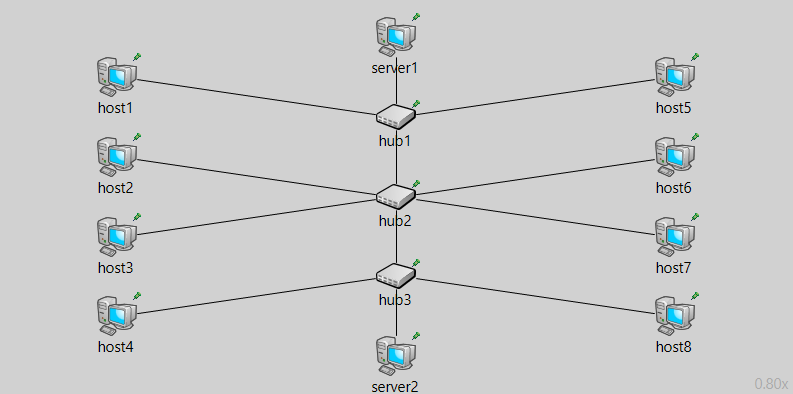
\includegraphics[width=0.6\linewidth]{screenshot001}
		\caption{Network Description of 1.1 parts a to c}
		\label{fig:screenshot001}
	\end{figure}
	
	\pagebreak
	
	The next step is to construct the initialization file(.ini). I added the mentioned configurations to each host and server and then established the needed frame transmissions. The code is shown in the following figure.
	
	\begin{figure}[!h]
		\centering
		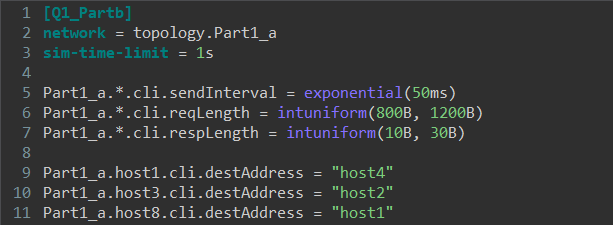
\includegraphics[width=0.6\linewidth]{screenshot002}
		\caption{Initialization code for the needed configurations}
		\label{fig:screenshot002}
	\end{figure}
	
	Then I simulated the Network.
	
	The results I got from the simulation are displayed in figures \ref{1} and \ref{2}.
	
	\begin{figure}[!h]
		\centering
		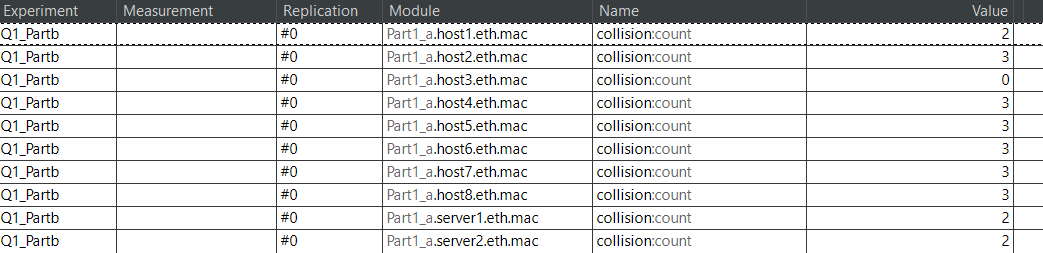
\includegraphics[width=0.6\linewidth]{1.1.b_col}
		\caption{The collision count in each node}
		\label{1}
	\end{figure}
	\begin{figure}[!h]
		\centering
		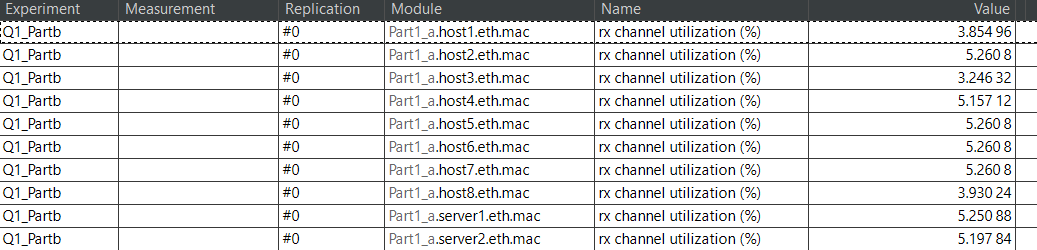
\includegraphics[width=0.6\linewidth]{1.1.b_util}
		\caption{Utilization of each node}
		\label{2}
	\end{figure}
	
	As we can see from the results, the total count of collisions and the mean utilization of the nodes were 24(2.4 average) and 4.75\% respectively.
	
	Theoretical calculations:
	
	\begin{center}
		$
		\vspace{0.1cm}
		\text{request transmission time} : \dfrac{1000B \times 8}{10 \times 10^6} = 0.8msec\linebreak
		\vspace{0.1cm}
		\text{response transmission time} : \dfrac{20B \times 8}{10 \times 10^6} = 0.016msec\linebreak
		\vspace{0.2cm}
		\text{request generation rate} : 3 \times \dfrac{1}{0.05} = 60 req/sec\linebreak
		\vspace{0.1cm}
		\text{total transmission bandwidth} : 60 \times (1000 + 20) \times 8 = 0.4896 Mbps\linebreak
		\vspace{0.1cm}
		\Rightarrow \text{channel utilization} : \dfrac{0.4896}{10} \times 100 \approx 4.9\% (\text{collision free})
		$
	\end{center}
	
	So as I derived the theoretical and simulation results are close to each other and the little difference is because of the randomness of the packet length and also the sending intervals. 
	
	\pagebreak
	
	\Large
	c)
	\large
	
	I changed the \textit{sendInterval} parameter to \textit{exponential(10ms)} and then repeated the process of the previous part.
	
	The obtained results:
	
	\begin{figure}[!h]
		\centering
		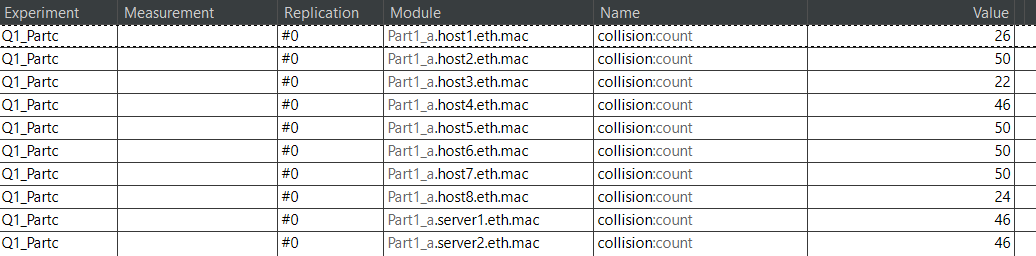
\includegraphics[width=0.6\linewidth]{1.1.c_col}
		\caption{The collision count in each node}
		\label{fig:1}
	\end{figure}
	\begin{figure}[!h]
		\centering
		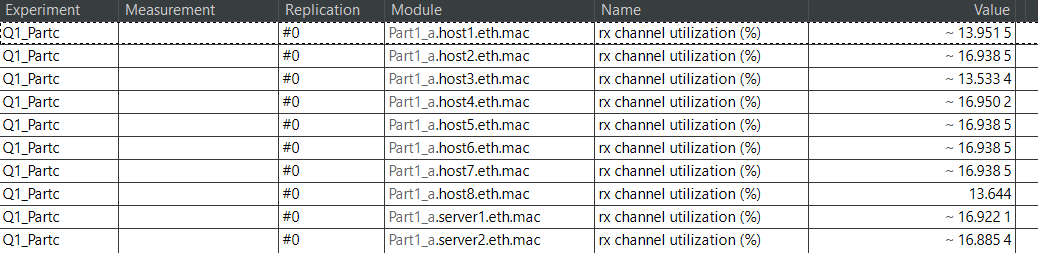
\includegraphics[width=0.6\linewidth]{1.1.c_util}
		\caption{Utilization of each node}
		\label{fig:2}
	\end{figure}
	
	It is observed that the total collisions went from 24 up to 410 and also the utilization rose to 15.96\%.
	
	The increase in the number of collisions is because the \textit{sendInterval} is decreased from 50msec to 10msec. This means the channel is now 5 times busier, and packets are far more likely to overlap in time, especially since each hub simply broadcasts to all ports.
	As the channel becomes busier, the chance that two nodes will transmit at nearly the same time rises exponentially, causing collision rates to grow remarkably.
	
	Theoretical calculations:
	
	\begin{center}
		$
		\vspace{0.1cm}
		\text{request transmission time} : \dfrac{1000B \times 8}{10 \times 10^6} = 0.8msec\linebreak
		\vspace{0.1cm}
		\text{response transmission time} : \dfrac{20B \times 8}{10 \times 10^6} = 0.016msec\linebreak
		\vspace{0.2cm}
		\text{request generation rate} : 3 \times \dfrac{1}{0.01} = 300 req/sec\linebreak
		\vspace{0.1cm}
		\text{total transmission bandwidth} : 300 \times (1000 + 20) \times 8 = 2.448 Mbps\linebreak
		\vspace{0.1cm}
		\Rightarrow \text{channel utilization} : \dfrac{2.448}{10} \times 100 \approx 24.48\% (\text{collision free})
		$
	\end{center}
	
	As obvious in the calculations, the ideal utilization(without any collisions) is 24.48\%. But in this case because we have a notable collision rate(unlike with the previous part where the collision rate was negligible) the actual utilization is less than the theoretical value.
	
	\pagebreak
	
	\Large
	d)
	\large
	
	Now in this part I changed the Ethernet Hubs into Ethernet Switches and then repeated the previous parts.
	
	\begin{figure}[!h]
		\centering
		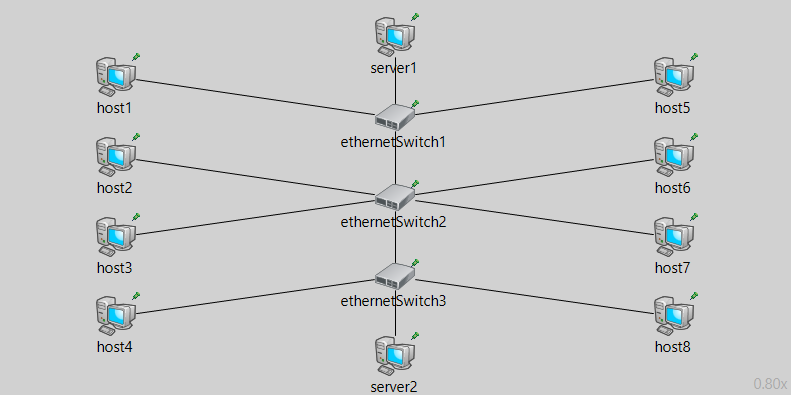
\includegraphics[width=0.6\linewidth]{screenshot003}
		\caption{Network description of 1.1 part d}
		\label{fig:screenshot003}
	\end{figure}
	
	\begin{figure}[!h]
		\centering
		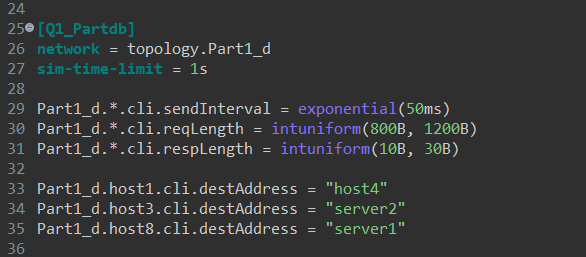
\includegraphics[width=0.6\linewidth]{screenshot004}
		\caption{Initialization code for the needed configurations}
		\label{fig:screenshot004}
	\end{figure}
	
	\Large
	\textit{sendInterval = exponential(50ms)}:
	\large
	
	\begin{figure}[!h]
		\centering
		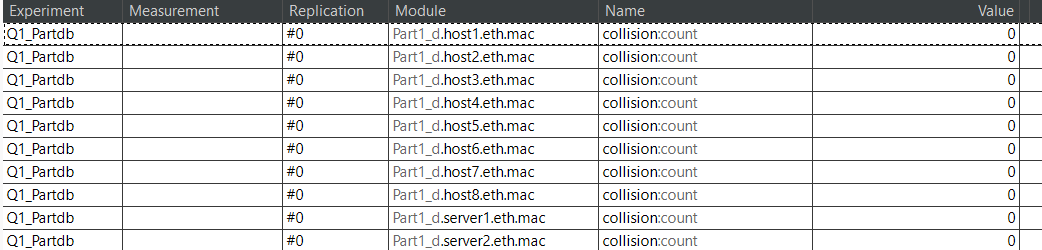
\includegraphics[width=0.7\linewidth]{1.1.db_col}
		\caption{The collision count in each node}
		\label{fig:1}
	\end{figure}
	
	\begin{figure}[!htb]
		\begin{minipage}{0.49\textwidth}
			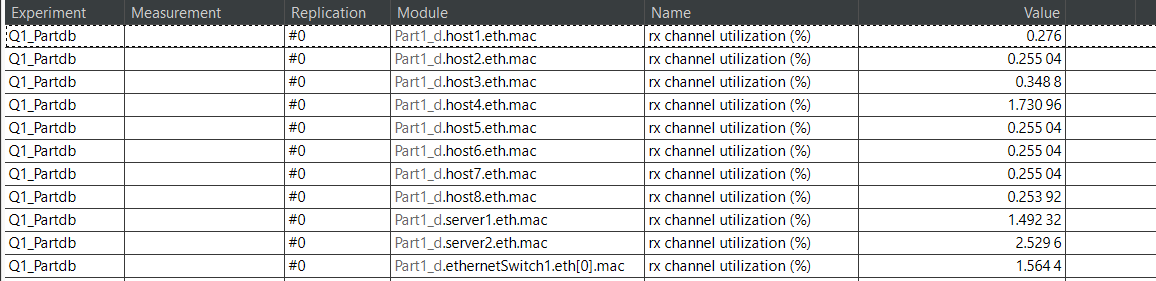
\includegraphics[width=\linewidth]{1.1.db_util1}
		\end{minipage}\hfill
		\begin{minipage}{0.49\textwidth}
			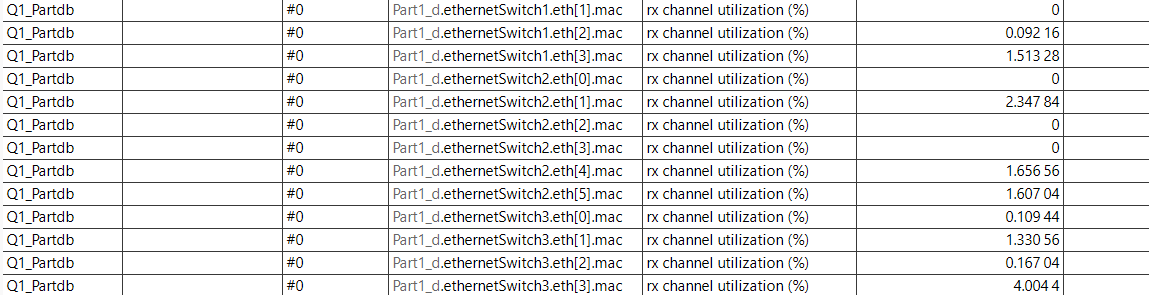
\includegraphics[width=\linewidth]{1.1.db_util2}
		\end{minipage}\hfill
		\caption{Utilization of each node}
		\label{2}
	\end{figure}
	
	\pagebreak
	
	\Large
	\textit{sendInterval = exponential(10ms)}:
	\large
	
	\begin{figure}[!h]
		\centering
		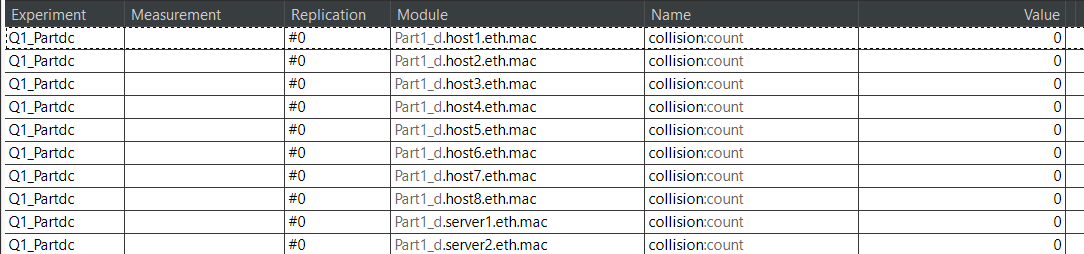
\includegraphics[width=0.7\linewidth]{1.1.dc_col}
		\caption{The collision count in each node}
		\label{fig:1}
	\end{figure}
	
	\begin{figure}[!htb]
		\begin{minipage}{0.49\textwidth}
			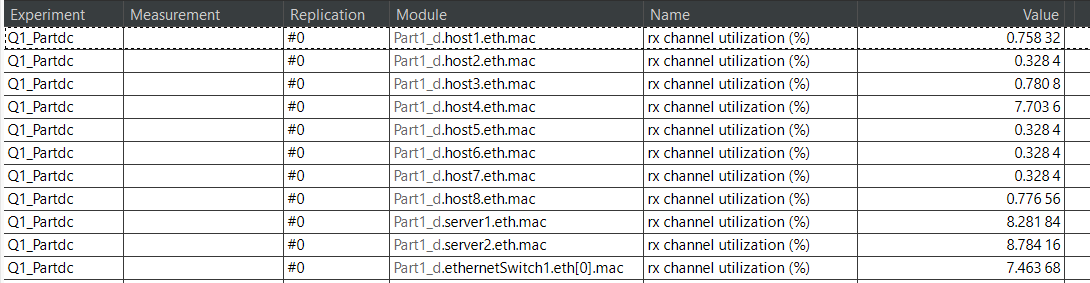
\includegraphics[width=\linewidth]{1.1.dc_util1}
		\end{minipage}\hfill
		\begin{minipage}{0.49\textwidth}
			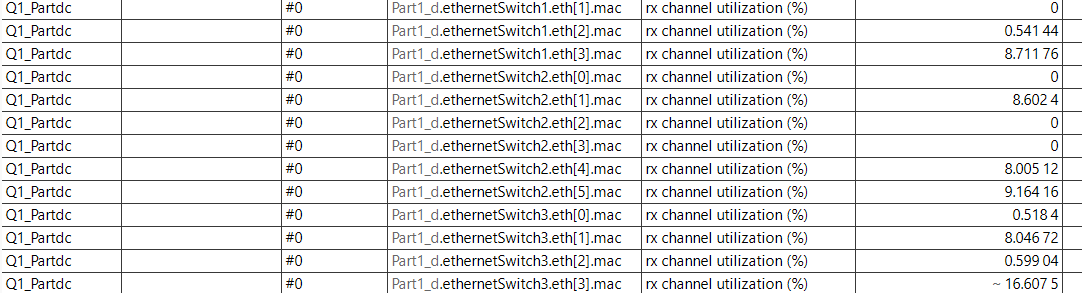
\includegraphics[width=\linewidth]{1.1.dc_util2}
		\end{minipage}\hfill
		\caption{Utilization of each node}
		\label{2}
	\end{figure}
	
	As seen from the results the collision rate is zero! This is because Ethernet Switches create isolated collision domains and each port is full-duplex and devices don't content for a shared medium anymore. Thus regardless of traffic rate the no collision will occur.
	
	The mean utilization of the nodes increased from nearly 0.9\% to around 4.1\% which is due to the traffic rate being 5 times higher in the latter case.
	
	\Large
	e)
	\large
	
	\begin{center}
		Flow of the frames in the Network using Ethernet Hubs:
	\end{center}
	
	\begin{figure}[!htb]
		\begin{minipage}{0.48\textwidth}
			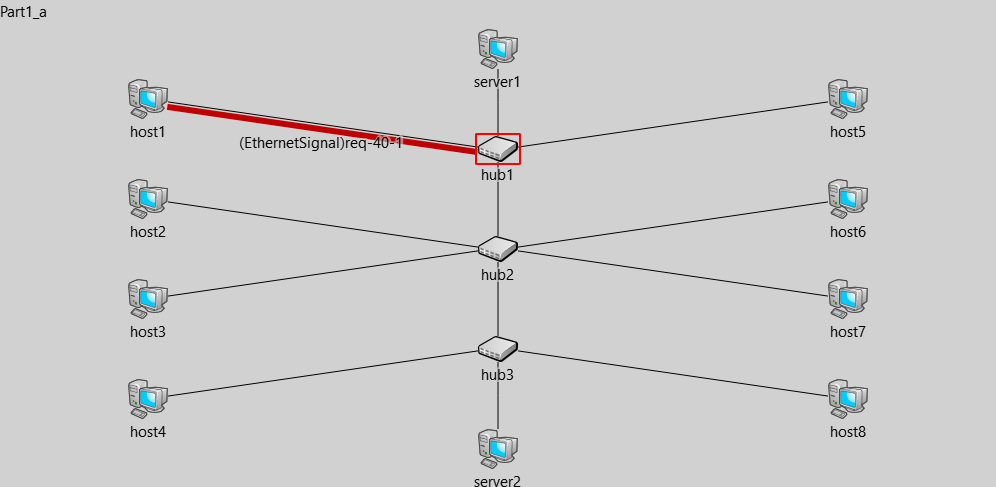
\includegraphics[width=\linewidth]{screenshot005}
		\end{minipage}\hfill
		\begin{minipage}{0.48\textwidth}
			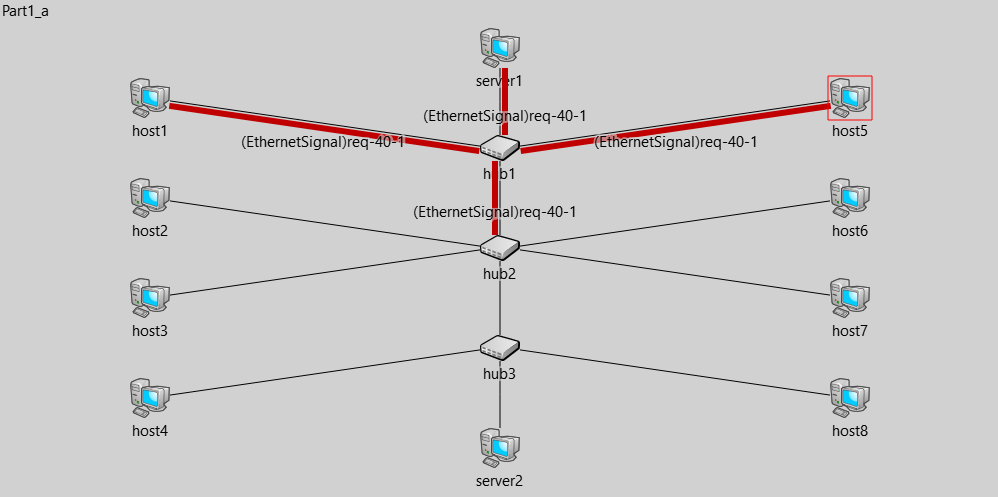
\includegraphics[width=\linewidth]{screenshot006}
		\end{minipage}\hfill
	\end{figure}
	\begin{figure}[!htb]
		\begin{minipage}{0.48\textwidth}
			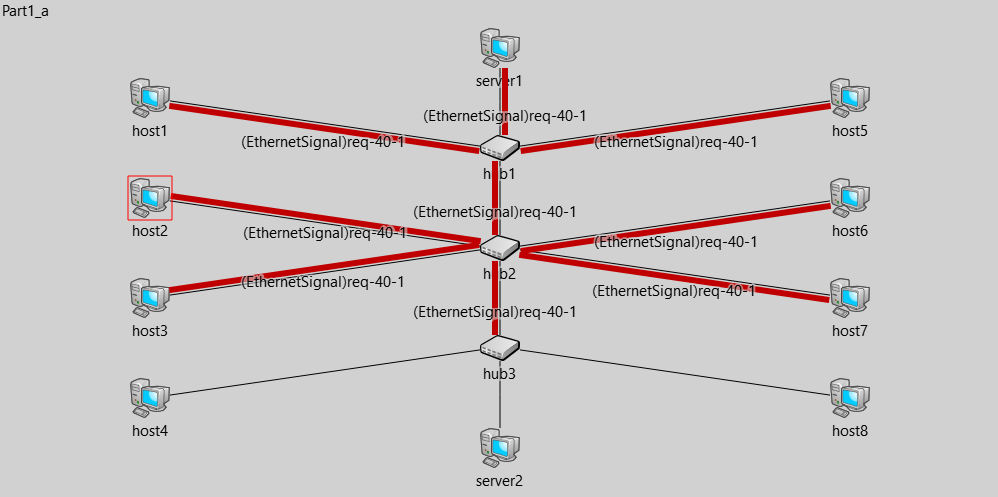
\includegraphics[width=\linewidth]{screenshot007}
		\end{minipage}\hfill
		\begin{minipage}{0.48\textwidth}
			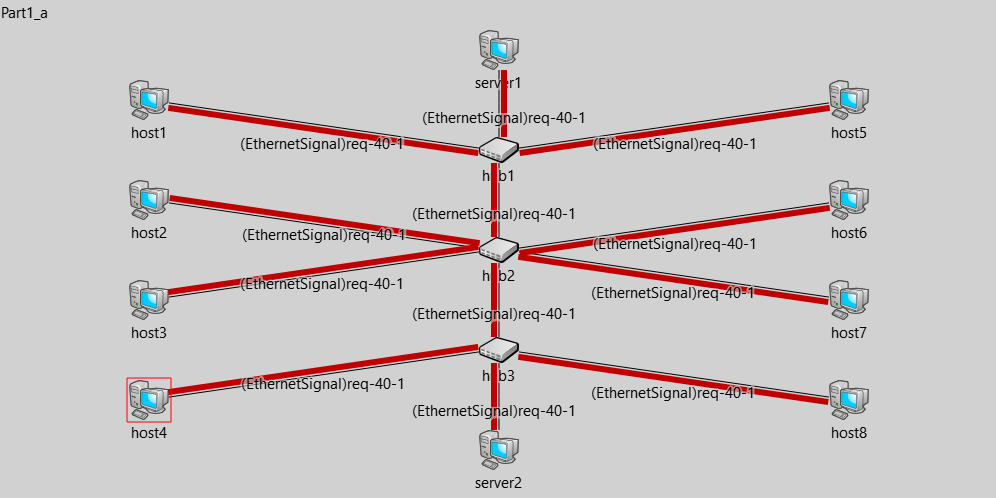
\includegraphics[width=\linewidth]{screenshot008}
		\end{minipage}\hfill
	\end{figure}
	
	\pagebreak
	
	\begin{figure}[!htb]
		\begin{minipage}{0.48\textwidth}
			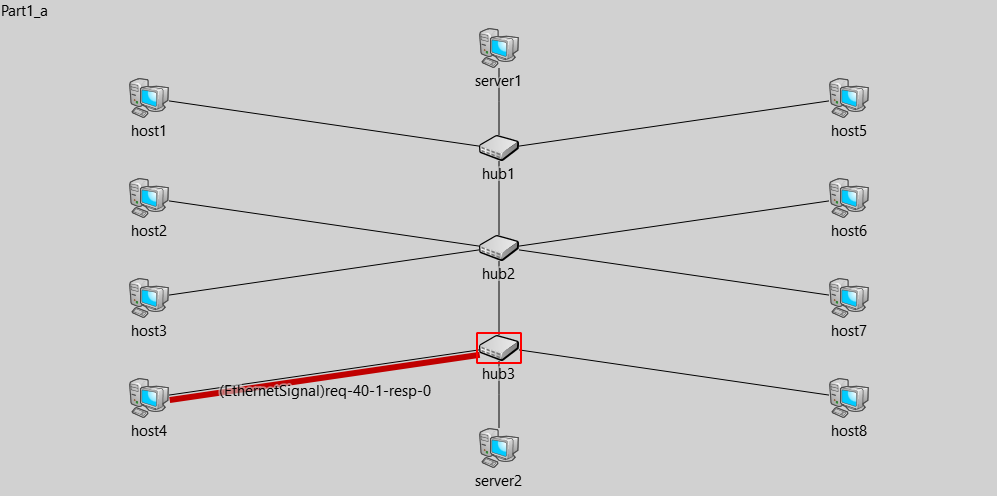
\includegraphics[width=\linewidth]{screenshot009}
		\end{minipage}\hfill
		\begin{minipage}{0.48\textwidth}
			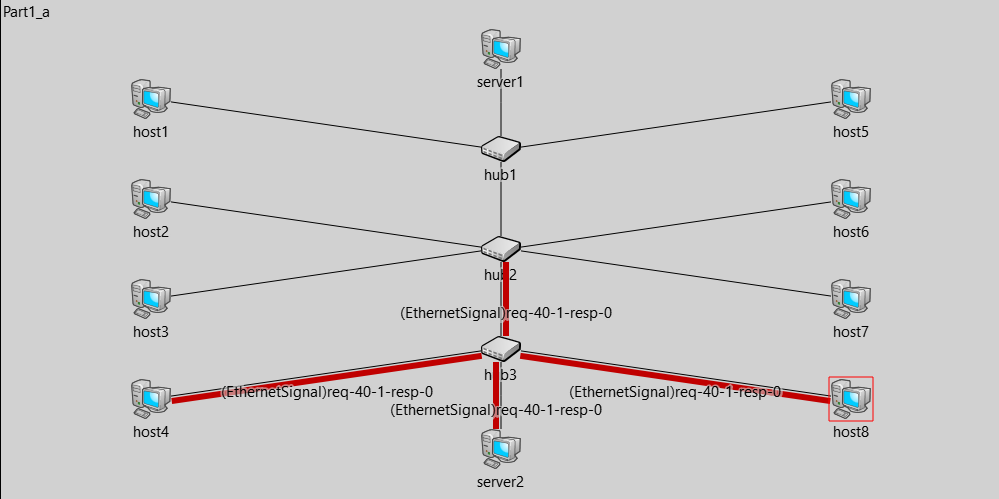
\includegraphics[width=\linewidth]{screenshot010}
		\end{minipage}\hfill
	\end{figure}
	\begin{figure}[!htb]
		\begin{minipage}{0.48\textwidth}
			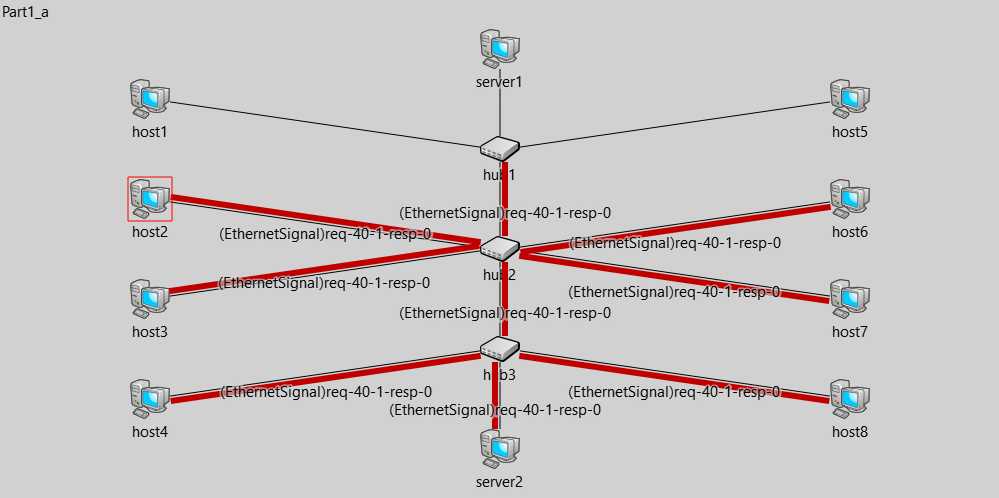
\includegraphics[width=\linewidth]{screenshot011}
		\end{minipage}\hfill
		\begin{minipage}{0.48\textwidth}
			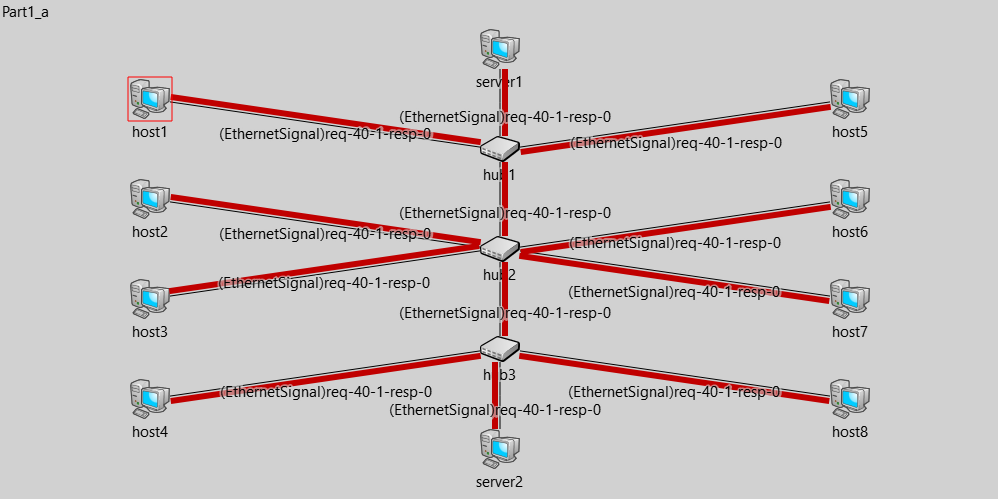
\includegraphics[width=\linewidth]{screenshot012}
		\end{minipage}\hfill
	\end{figure}
	
	As we can see in the first case, the Hubs send the signal they hear to all other ports of them each single time and they do not learn the host addresses.
	
	\begin{center}
		Flow of the frames in the Network using Ethernet Switches
	\end{center}
	
	\begin{figure}[!htb]
		\begin{minipage}{0.48\textwidth}
			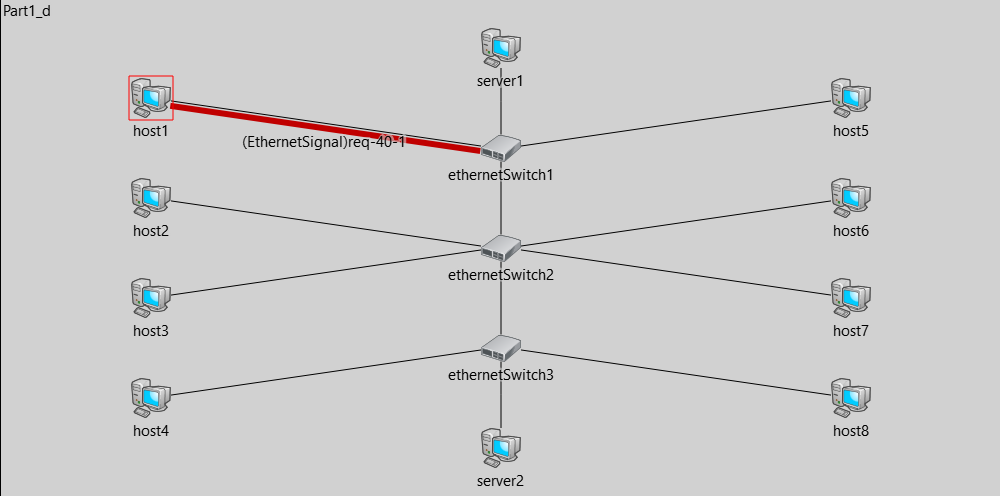
\includegraphics[width=\linewidth]{screenshot013}
		\end{minipage}\hfill
		\begin{minipage}{0.48\textwidth}
			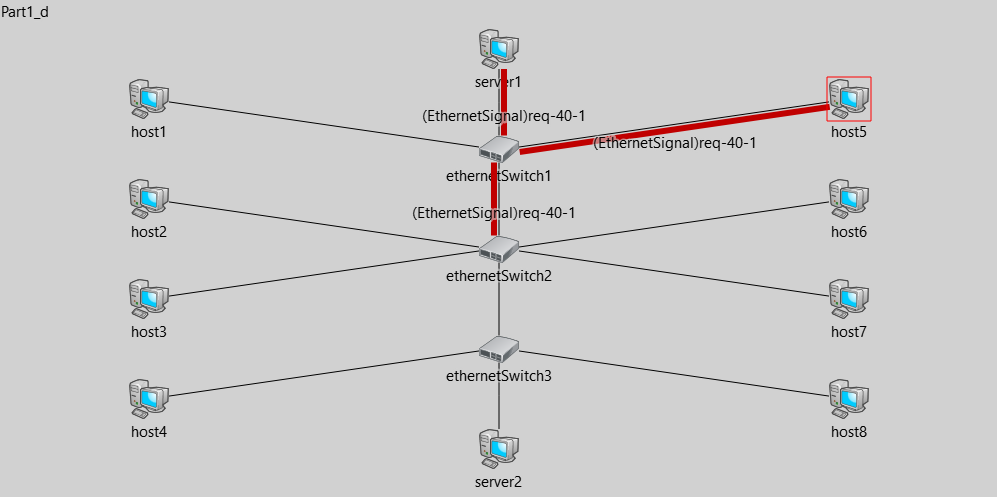
\includegraphics[width=\linewidth]{screenshot014}
		\end{minipage}\hfill
	\end{figure}
	\begin{figure}[!htb]
		\begin{minipage}{0.48\textwidth}
			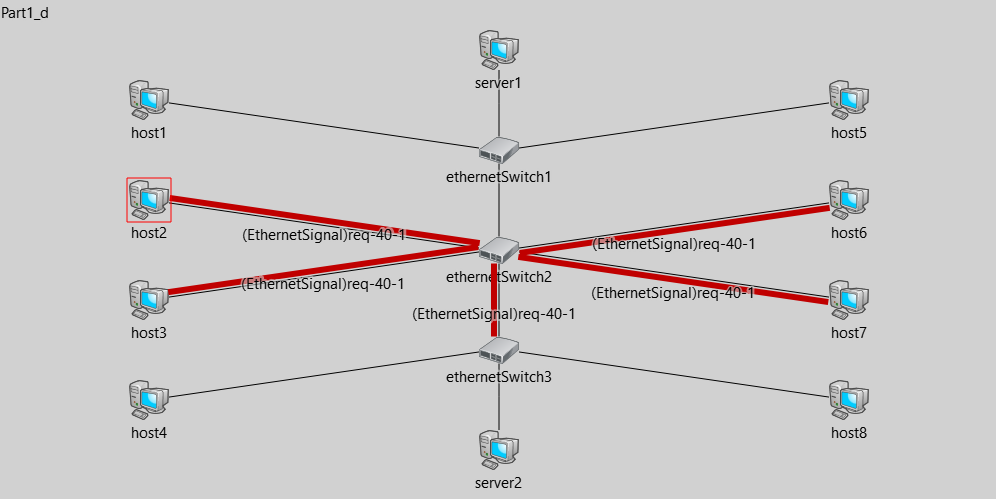
\includegraphics[width=\linewidth]{screenshot015}
		\end{minipage}\hfill
		\begin{minipage}{0.48\textwidth}
			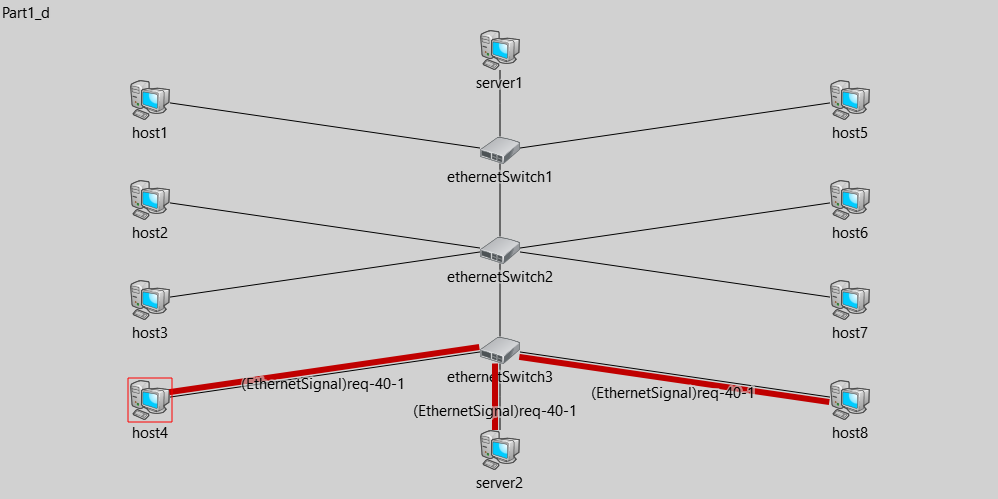
\includegraphics[width=\linewidth]{screenshot016}
		\end{minipage}\hfill
	\end{figure}
	\begin{figure}[!htb]
		\begin{minipage}{0.48\textwidth}
			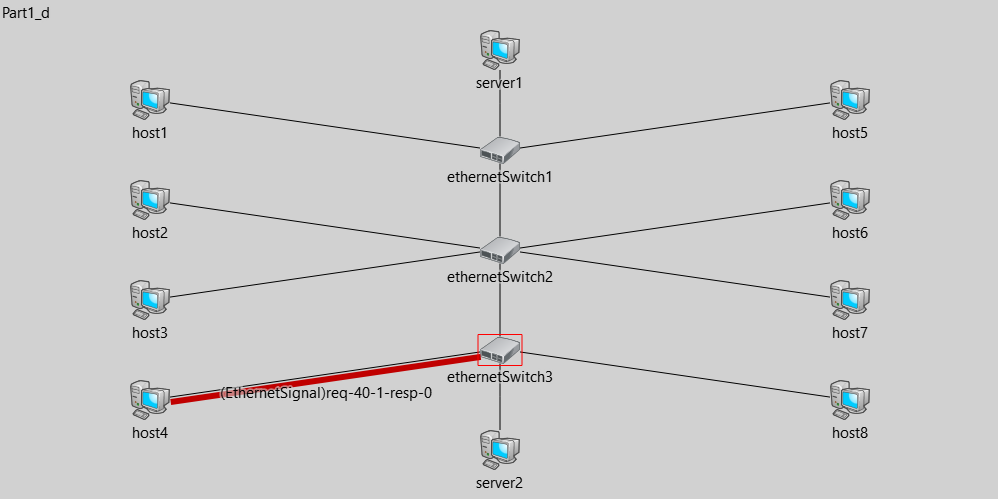
\includegraphics[width=\linewidth]{screenshot017}
		\end{minipage}\hfill
		\begin{minipage}{0.48\textwidth}
			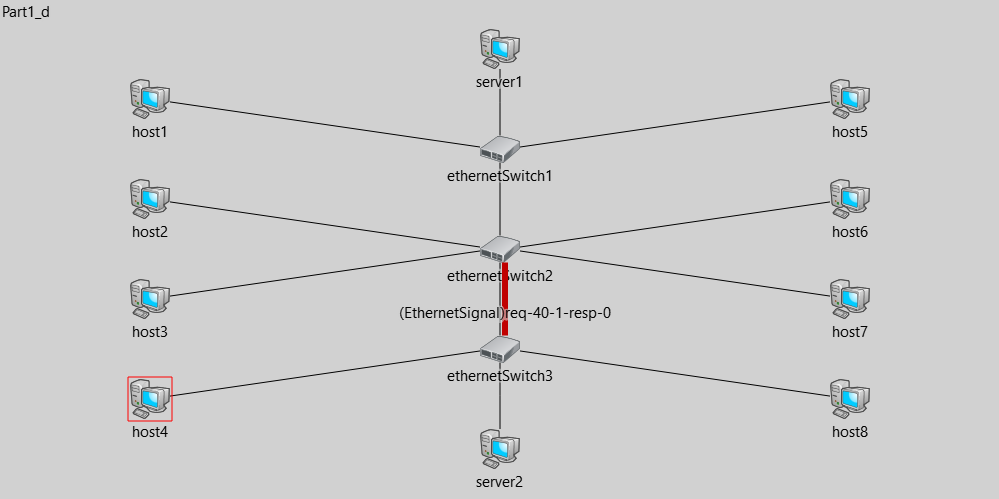
\includegraphics[width=\linewidth]{screenshot018}
		\end{minipage}\hfill
	\end{figure}
	
	\pagebreak
	
	\begin{figure}[!htb]
		\begin{minipage}{0.48\textwidth}
			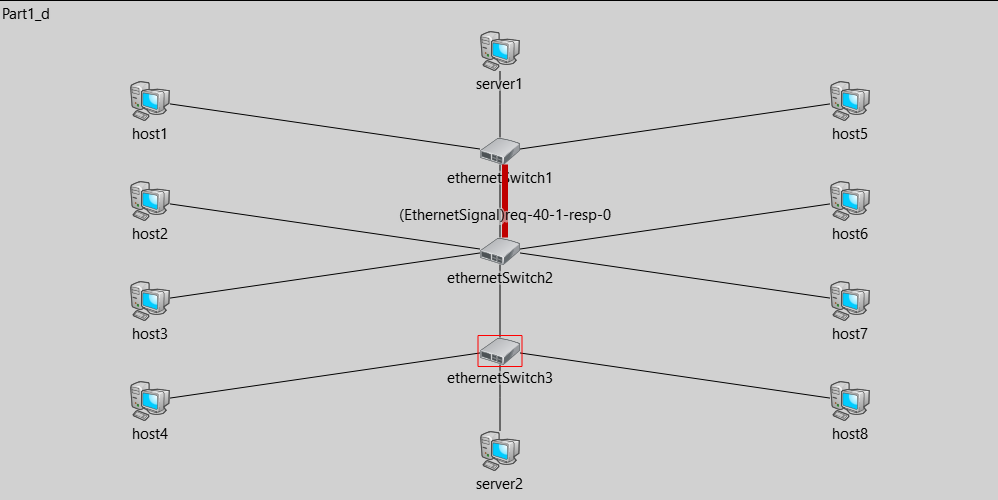
\includegraphics[width=\linewidth]{screenshot019}
		\end{minipage}\hfill
		\begin{minipage}{0.48\textwidth}
			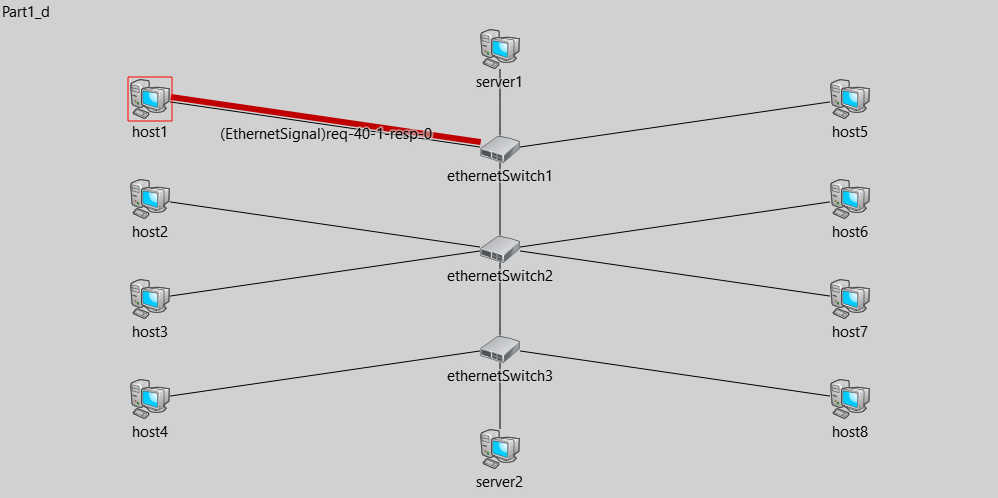
\includegraphics[width=\linewidth]{screenshot020}
		\end{minipage}\hfill
	\end{figure}
	\begin{figure}[!htb]
		\begin{minipage}{0.48\textwidth}
			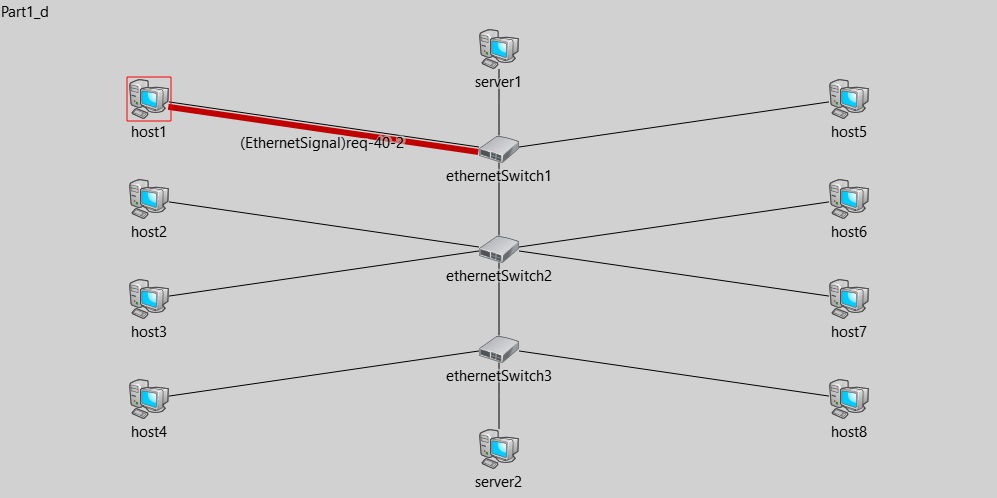
\includegraphics[width=\linewidth]{screenshot021}
		\end{minipage}\hfill
		\begin{minipage}{0.48\textwidth}
			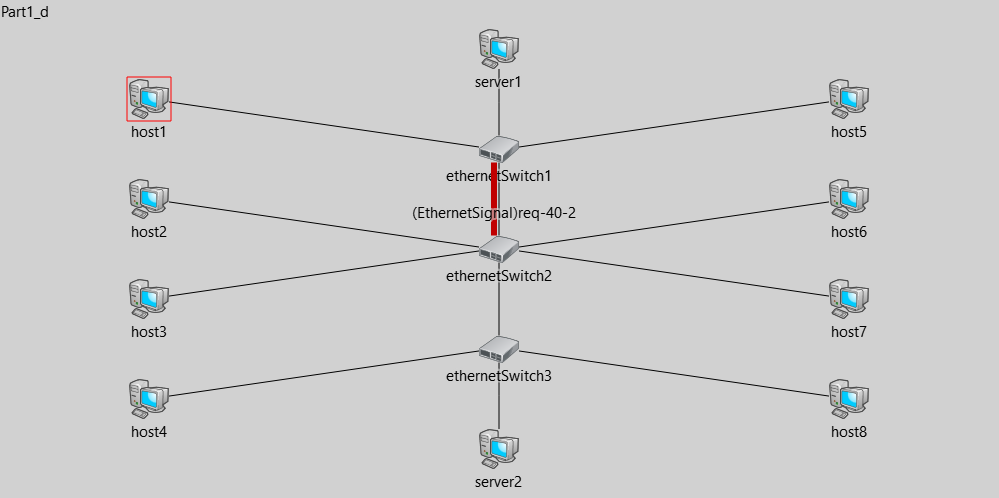
\includegraphics[width=\linewidth]{screenshot022}
		\end{minipage}\hfill
	\end{figure}
	\begin{figure}[!htb]
		\begin{minipage}{0.48\textwidth}
			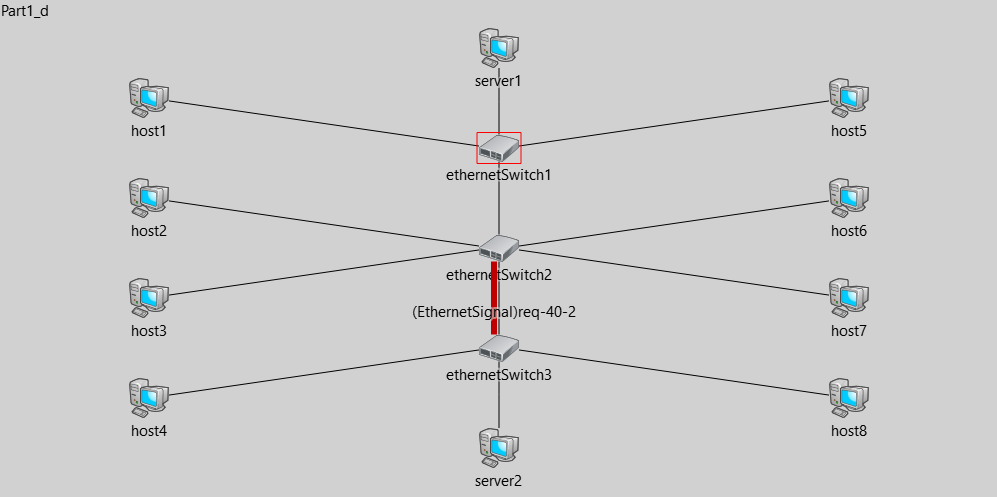
\includegraphics[width=\linewidth]{screenshot023}
		\end{minipage}\hfill
		\begin{minipage}{0.48\textwidth}
			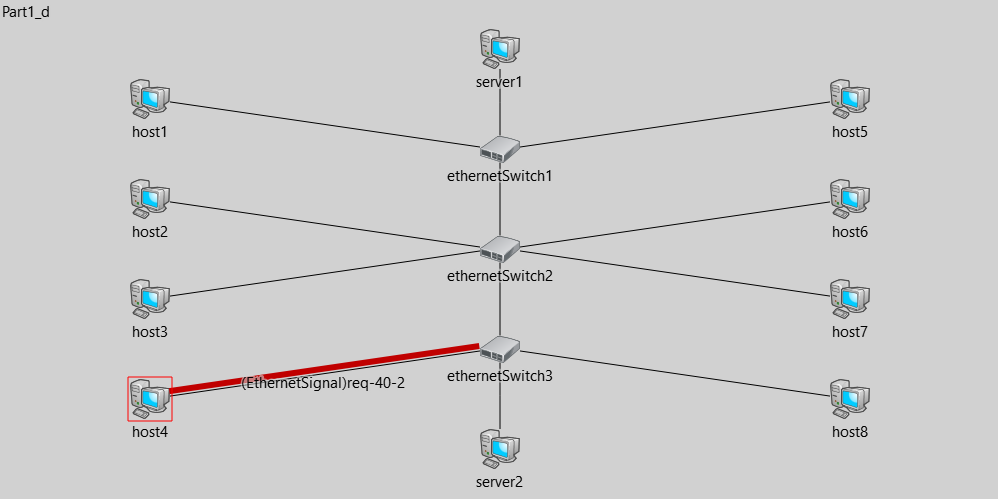
\includegraphics[width=\linewidth]{screenshot024}
		\end{minipage}\hfill
	\end{figure}
	\begin{figure}[!htb]
		\begin{minipage}{0.48\textwidth}
			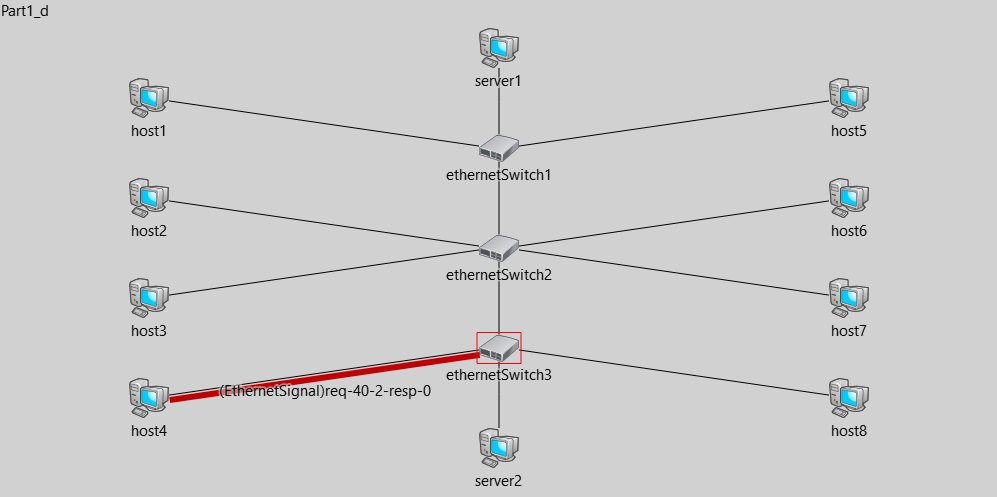
\includegraphics[width=\linewidth]{screenshot025}
		\end{minipage}\hfill
		\begin{minipage}{0.48\textwidth}
			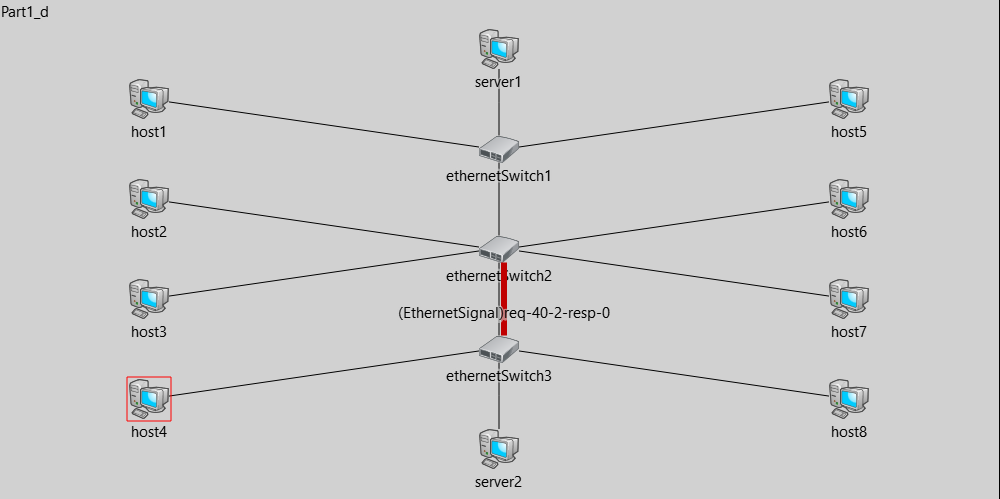
\includegraphics[width=\linewidth]{screenshot026}
		\end{minipage}\hfill
	\end{figure}
	\begin{figure}[!htb]
		\begin{minipage}{0.48\textwidth}
			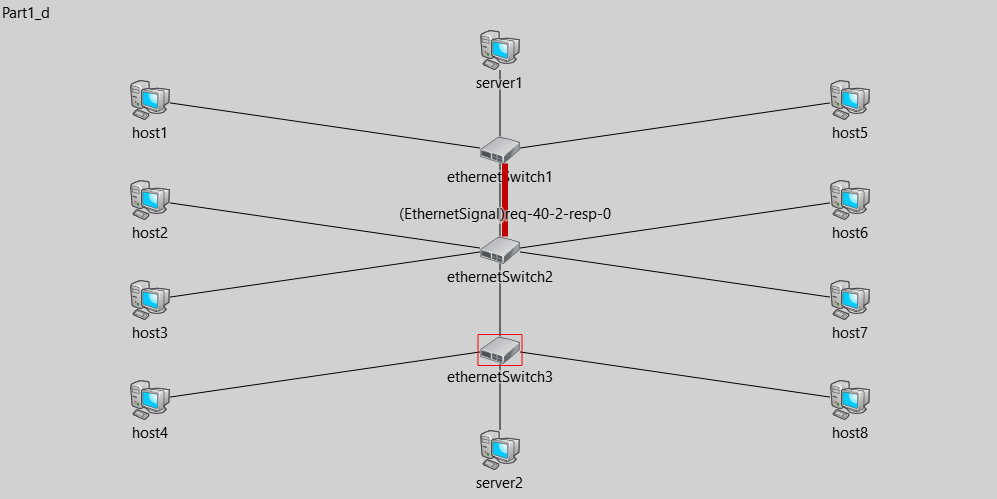
\includegraphics[width=\linewidth]{screenshot027}
		\end{minipage}\hfill
		\begin{minipage}{0.48\textwidth}
			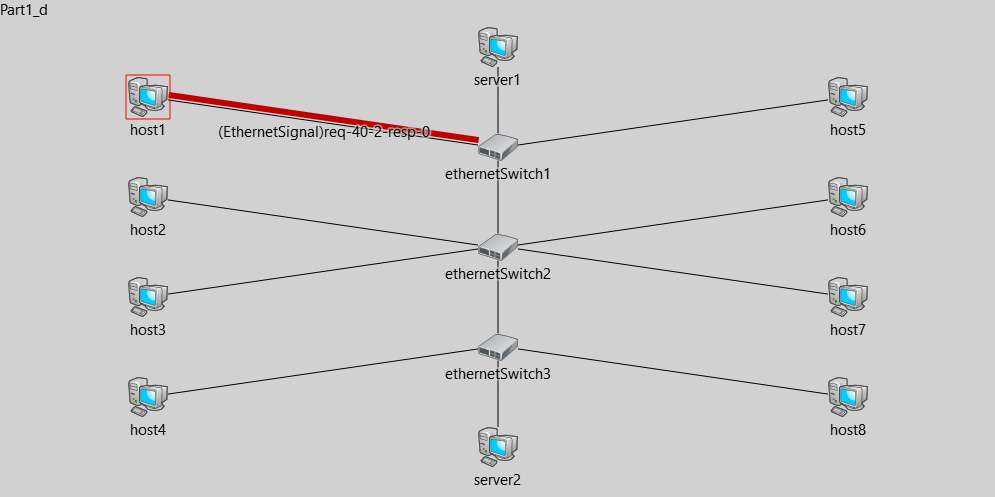
\includegraphics[width=\linewidth]{screenshot028}
		\end{minipage}\hfill
	\end{figure}
	
	The Switches on the other hand, learn the address of the hosts transmitting frames to them in the first transmission and from that point they do not send the receiving frames to all other ports and they just transmit the frame in the right path.
	
	So we observed the explanations provided in part (a) in simulation.
	
	\subsection{CSMA/CD}
	
	In this part we ought to investigate CSMA/CD behavior. The topology of the network is shown in Figure \ref{fig:screenshot032}.
	
	\begin{figure}[!h]
		\centering
		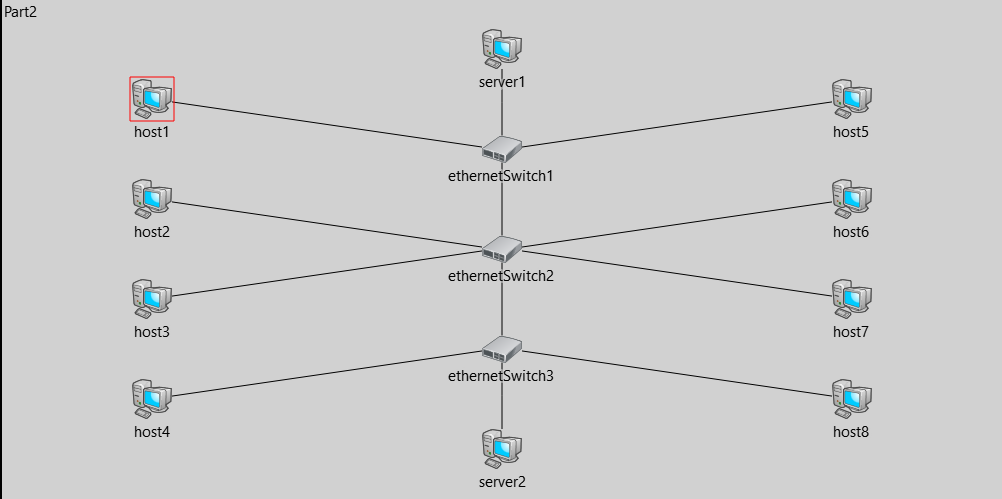
\includegraphics[width=0.7\linewidth]{screenshot032}
		\caption{Network description of 1.2}
		\label{fig:screenshot032}
	\end{figure}
	
	It is demanded that the odd-numbered hosts send requests to \textit{server1} and the even-numbered ones to \textit{server2}. Also I should make sure that the odd-numbered hosts do not support CSMA/CD but other nodes use CSMA/CD.
	
	The code for this simulation configuration is provided in the following figure.
	
	\begin{figure}[!h]
		\centering
		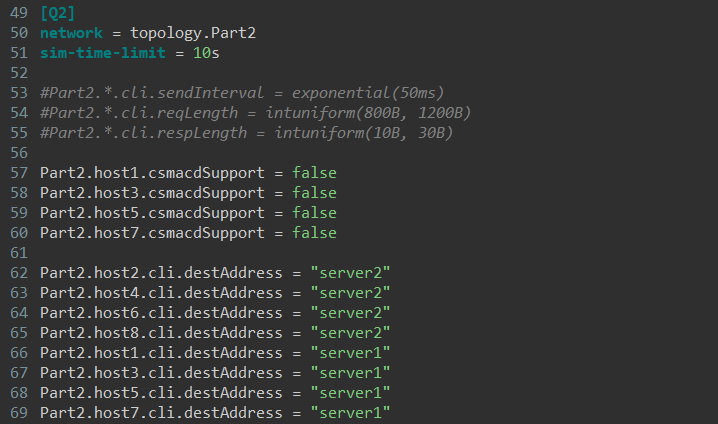
\includegraphics[width=0.7\linewidth]{screenshot033}
		\caption{Initialization code for the needed configurations}
		\label{fig:screenshot033}
	\end{figure}
	
	I set the simulation time to 10 seconds so that there is enough time for several transmissions from each node.
	
	\pagebreak
	
	The results were as below.
	
	\begin{figure}[!h]
		\centering
		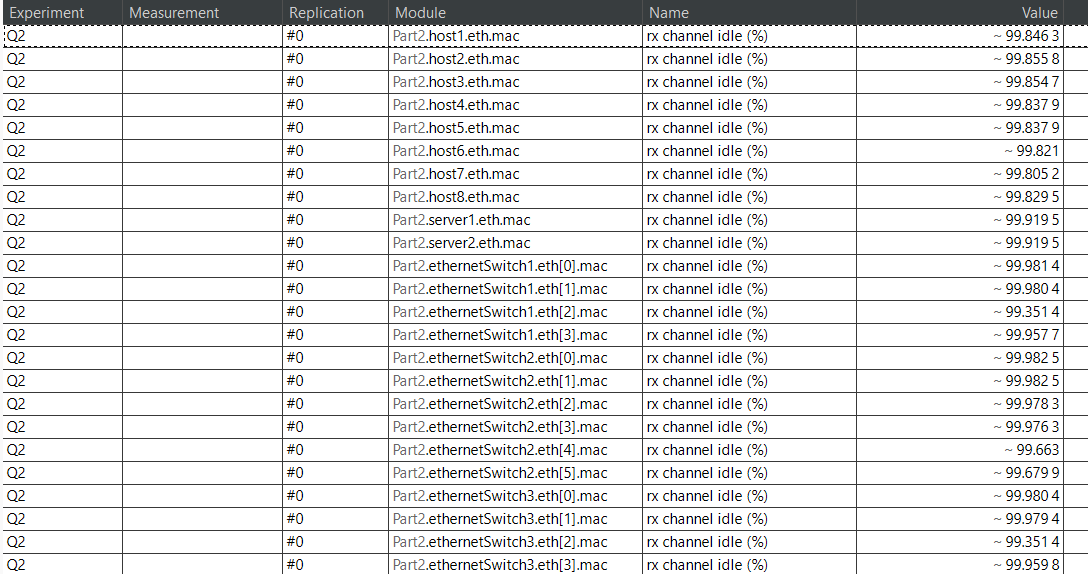
\includegraphics[width=0.7\linewidth]{screenshot029}
		\caption{rx channel idle}
		\label{fig:screenshot029}
	\end{figure}
	\begin{figure}[!h]
		\centering
		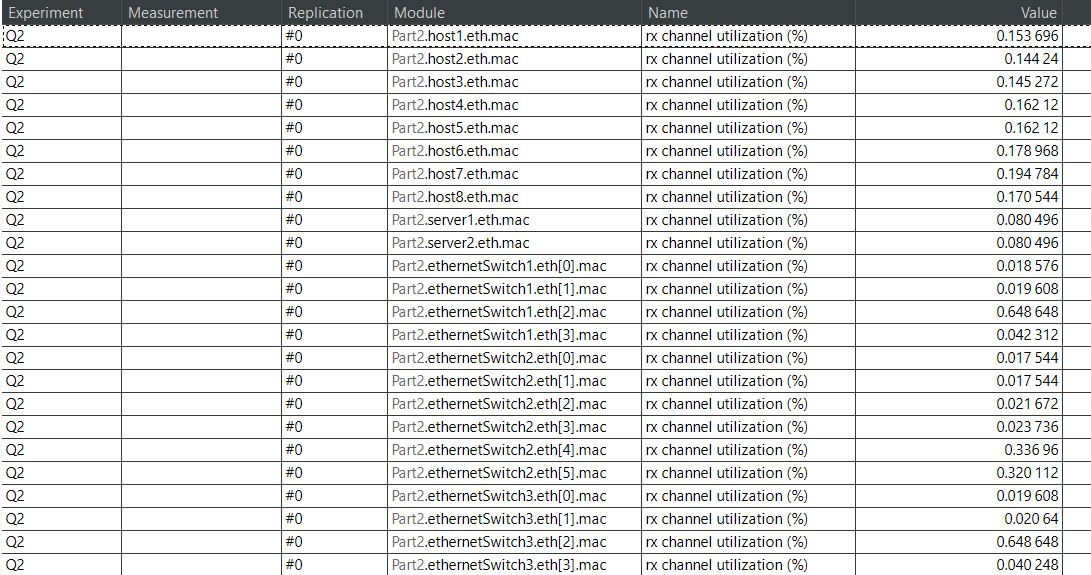
\includegraphics[width=0.7\linewidth]{screenshot030}
		\caption{rx channel utilization}
		\label{fig:screenshot030}
	\end{figure}
	\begin{figure}[!h]
		\centering
		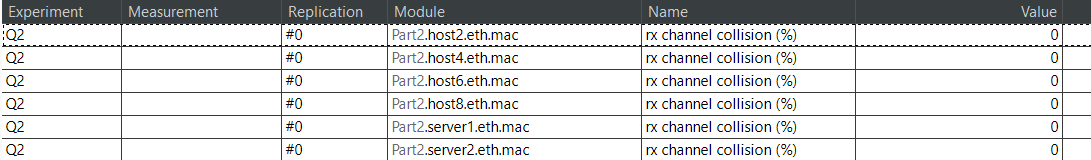
\includegraphics[width=0.7\linewidth]{screenshot031}
		\caption{rx channel collision}
		\label{fig:screenshot031}
	\end{figure}
	
	As we observed, the \textit{rx channel collision} is not measured in the odd-numbered nodes because they do not support collision detection.
	
	From the results we see that the rx channel of each node is almost always idle(nearly 99\% in each node) and therefore the \textit{rx channel utilization} is extremely low in all of the nodes(less than 1\%).
	
	Also no collision is detected in the node supporting CSMA/CD because we have used \textit{Ethernet Switched} and they use isolated full-duplex collision domains in each port.
	
	\pagebreak
	
	\subsection{MAC Address}
	\Large
	a)
	\large
	
	In this part we need configure the MAC addresses as given and then display the assigned addresses during simulation. I also have to capture and report each switch's MAC address table.
	
	\begin{figure}[!h]
		\centering
		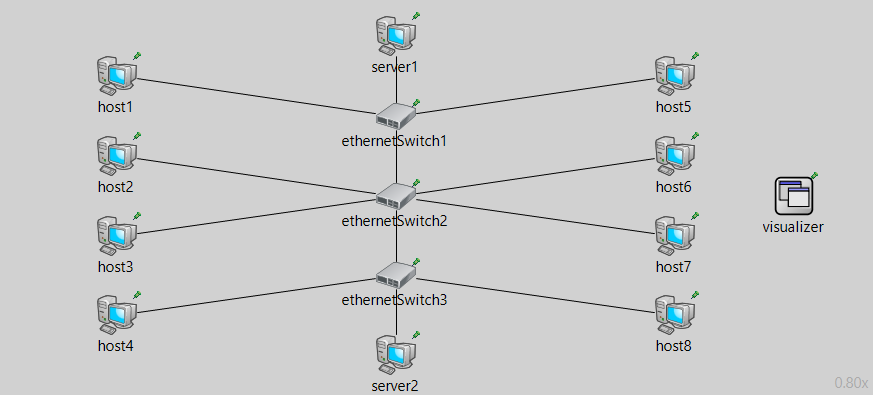
\includegraphics[width=0.7\linewidth]{screenshot035}
		\caption{Network description of 1.3}
		\label{fig:screenshot035}
	\end{figure}
	\begin{figure}[!h]
		\centering
		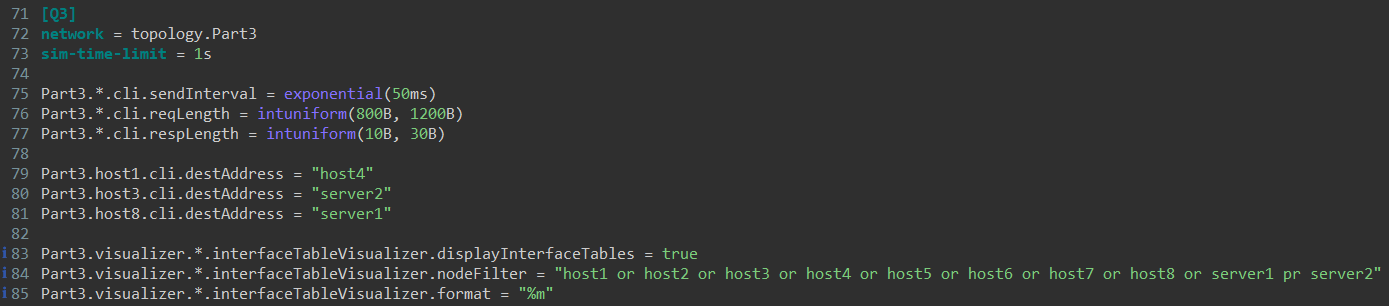
\includegraphics[width=0.7\linewidth]{screenshot034}
		\caption{Initialization code for the needed configurations}
		\label{fig:screenshot034}
	\end{figure}
	
	The first step was to set the wanted MAC address to each node. In order to do this I used the code line \textit{@macAddress}. This method didn't work and the MAC addresses were not assigned correctly.
	
	\begin{figure}[!h]
		\centering
		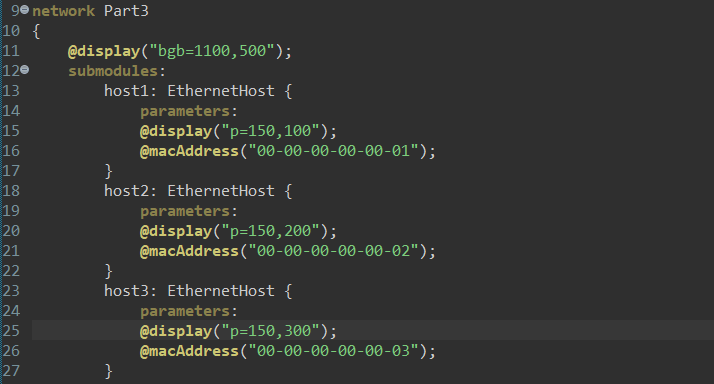
\includegraphics[width=0.7\linewidth]{screenshot036}
		\caption{}
		\label{fig:screenshot036}
	\end{figure}
	
	\pagebreak
	
	Then I decided to set the addresses in the initialization file. The added code to the initializations is displayed in Figure \ref{fig:screenshot037}.
	
	\begin{figure}[!h]
		\centering
		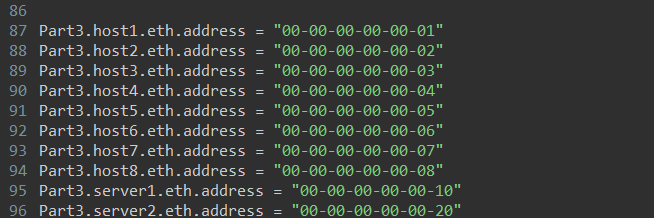
\includegraphics[width=0.7\linewidth]{screenshot037}
		\caption{The code added to the initialization file}
		\label{fig:screenshot037}
	\end{figure}
	
	The resulting network from simulation is shown in the figure below.
	
	\begin{figure}[!h]
		\centering
		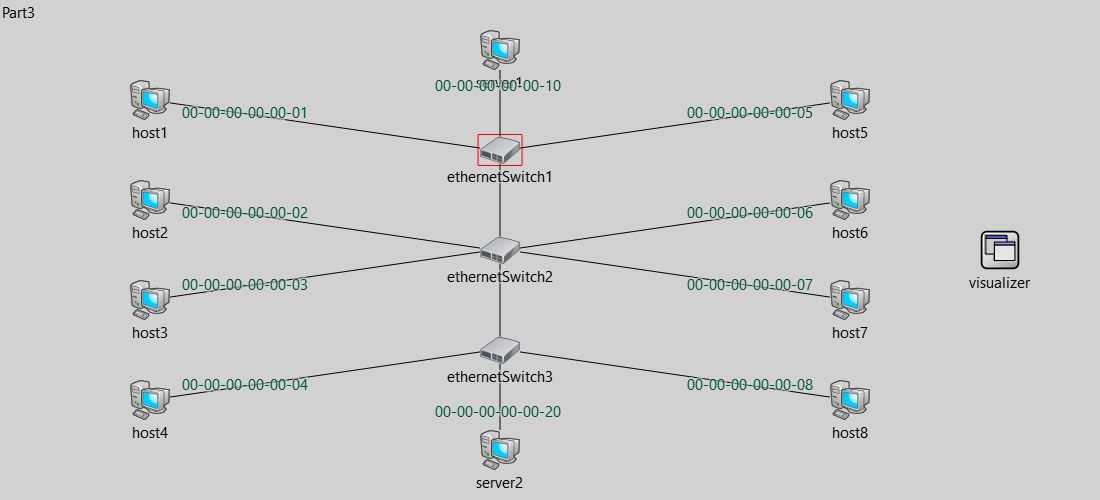
\includegraphics[width=0.7\linewidth]{screenshot038}
		\caption{}
		\label{fig:screenshot038}
	\end{figure}
	
	The MAC address of each node is displayed correctly which is what we desired.
	
	\Large
	b)
	\large
	
	After simulating the network, I captured the \textit{forwardingTable} in the \textit{macTable} property of each
	\textit{EthernetSwitch}. You can see the resulting tables for each Switch in the following figures.
	
	\vspace{1cm}
	
	\begin{figure}[!h]
		\centering
		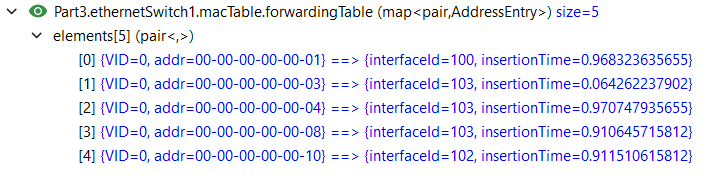
\includegraphics[width=0.7\linewidth]{screenshot039}
		\caption{MAC address table of \textit{EthernetSwitch1}}
		\label{fig:screenshot039}
	\end{figure}
	
	\pagebreak
	
	\begin{figure}[!h]
		\centering
		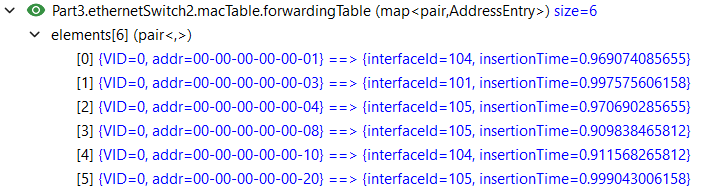
\includegraphics[width=0.7\linewidth]{screenshot040}
		\caption{MAC address table of \textit{EthernetSwitch2}}
		\label{fig:screenshot040}
	\end{figure}
	\begin{figure}[!h]
		\centering
		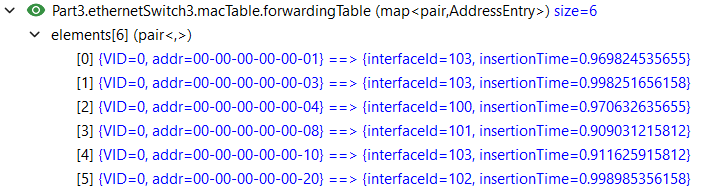
\includegraphics[width=0.7\linewidth]{screenshot041}
		\caption{MAC address table of \textit{EthernetSwitch3}}
		\label{fig:screenshot041}
	\end{figure}
	
	As it is obvious from the results, the addresses are accurately saved in the MAC address tables.
	\pagebreak
	
	\section{VLAN}
	\Large
	a)
	\large
	
	A Virtual LAN (VLAN) is a logical grouping of devices on a local area network (LAN) that are configured to communicate as if they are on the same physical network, regardless of their actual physical location. VLANs allow network administrators to segment a network into multiple, smaller networks, improving performance, security, and management.
	
	advantages of VLAN:
	
	Improved Security,
	Better Network Performance,
	Simplified Management,
	Flexibility and Scalability,
	and Reduced Costs
	
	\Large
	b,c)
	\large
	
	The network description for this problem is shown in the following figure.
	
	\begin{figure}[!h]
		\centering
		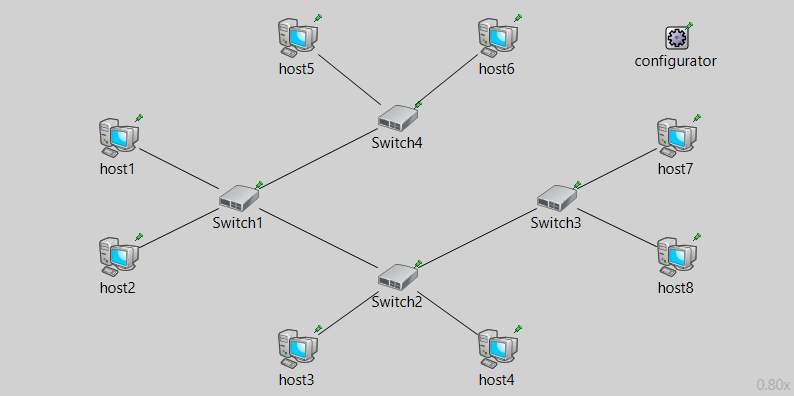
\includegraphics[width=0.7\linewidth]{screenshot045}
		\caption{Network description of problem 2}
		\label{fig:screenshot045}
	\end{figure}
	
	8 \textit{StandardHosts} are transmitting frames and are connected to each other using 4 \textit{EthernetSwitches}. The links connecting the hosts to switches and switches to each other are all 10 meter \textit{Eth10M}s.
	
	Using the VLAN example provided in inet, I assigned the needed vlanIDs to the hosts and also set the accepted in and out vlanIDs for each switch using the codes below in the \textit{.ini} file.
	
	\begin{figure}[!h]
		\centering
		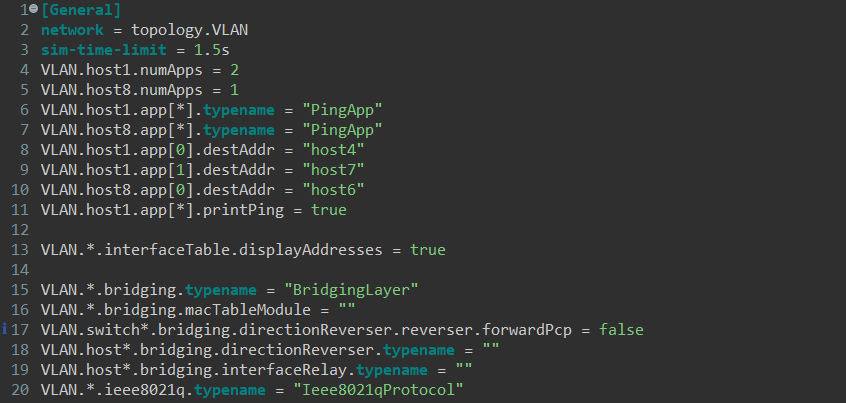
\includegraphics[width=0.7\linewidth]{screenshot044}
		\caption{Base configurations needed for VLANs and PingApp}
		\label{fig:screenshot044}
	\end{figure}
	
	\pagebreak
	
	\begin{figure}[!h]
		\centering
		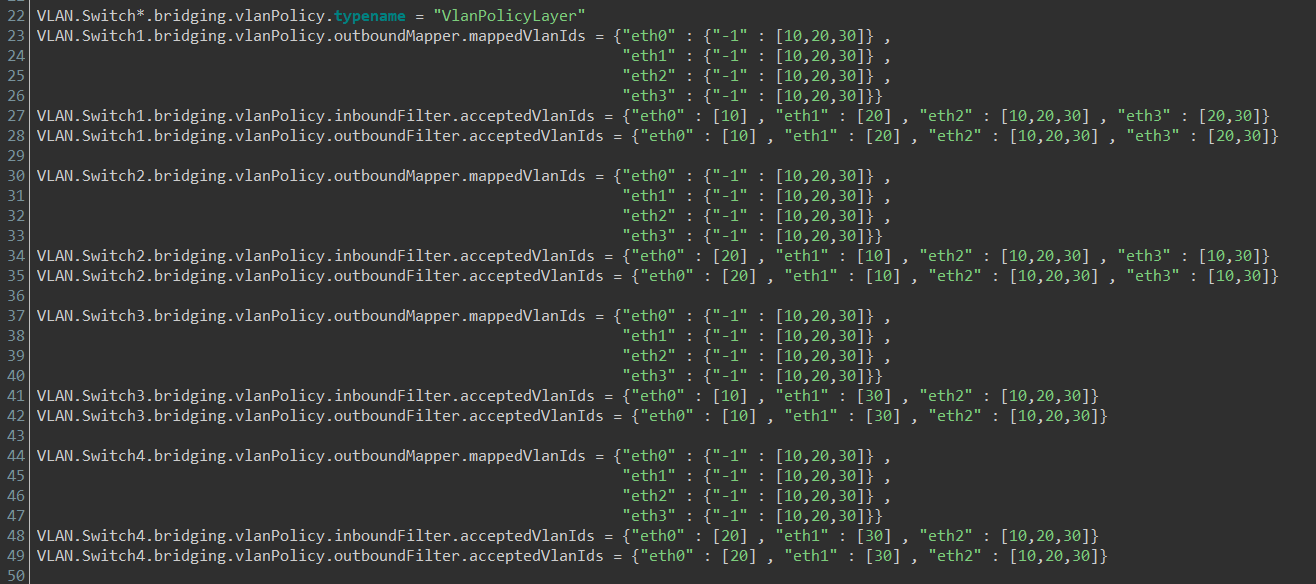
\includegraphics[width=0.7\linewidth]{screenshot043}
		\caption{Switch configurations}
		\label{fig:screenshot043}
	\end{figure}
	
	\begin{figure}[!h]
		\centering
		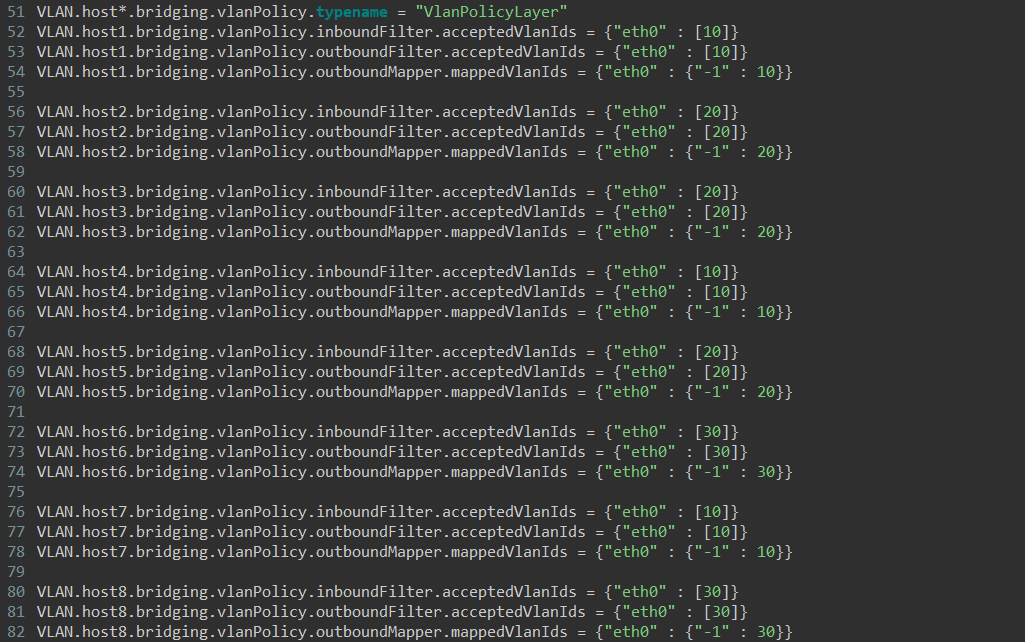
\includegraphics[width=0.7\linewidth]{screenshot042}
		\caption{Host configurations}
		\label{fig:screenshot042}
	\end{figure}
	
	Using the codes in the preceding figures, I determined the acceptable input and output vlanIDs for each switch.
	
	I learned from the inet vlan example that the code works like this:
	\begin{center}
		\textit{VLAN.host*.bridging.vlanPolicy.typename = "VlanPolicyLayer"}
	\end{center}
	This line applies the \textit{VlanPolicyLayer} to all hosts. It ensures that the hosts will also use VLAN filtering and mapping rules.
	
	\begin{center}
		\textit{VLAN.host1.bridging.vlanPolicy.inboundFilter.acceptedVlanIds = \{"eth0" : [10]\}}
	\end{center}
	This line specifies that \textit{host1} will only accept traffic tagged with vlanID 10 on its \textit{eth0} interface. Any traffic tagged with other vlanIDs will be rejected.
	
	\begin{center}
		\textit{VLAN.host1.bridging.vlanPolicy.outboundFilter.acceptedVlanIds = \{"eth0" : [10]\}}
	\end{center}
	This line ensures that \textit{host1} only sends traffic tagged with vlanID 10 on its \textit{eth0} interface. Any traffic with other VLAN tags will be discarded.
	
	\pagebreak
	
	\begin{center}
		\textit{VLAN.host1.bridging.vlanPolicy.outboundMapper.mappedVlanIds = \{"eth0" : \{"-1" : 10\}\}}
	\end{center}
	This line tells \textit{host1} to tag all outgoing traffic from its \textit{eth0} interface with vlanID 10. The -1 here means that all outgoing traffic will be tagged with VLAN 10.
	
	\begin{center}
		\textit{VLAN.Switch1.bridging.vlanPolicy.inboundFilter.acceptedVlanIds = \{"eth0" : [10] ,\\ "eth1" : [20] , "eth2" : [10,20,30] , "eth3" : [20,30]\}}
	\end{center}
	This line specifies which vlanIDs are accepted for incoming traffic on each of \textit{Switch1}'s interfaces.
	
	\begin{center}
		\textit{VLAN.Switch1.bridging.vlanPolicy.outboundFilter.acceptedVlanIds = \{"eth0" : [10] ,\\ "eth1" : [20] , "eth2" : [10,20,30] , "eth3" : [20,30]\}}
	\end{center}
	This line specifies which vlanIDs can be sent out on each of \textit{Switch1}'s interfaces:
	
	On \textit{eth0}, only VLAN 10 traffic is forwarded.
	
	On \textit{eth1}, only VLAN 20 traffic is forwarded.
	
	On \textit{eth2}, VLANs 10, 20, and 30 are forwarded.
	
	On \textit{eth3}, VLANs 20 and 30 are forwarded.
	
	\Large
	d)
	\large
	
	Now is the time to analyze the packet flow in the network and see how the packets are being transmitted.
	
	\begin{center}
		packet flow for \textit{host1} $\rightarrow$ \textit{host4} communication
	\end{center}
	
	\begin{figure}[!htb]
		\begin{minipage}{0.49\textwidth}
			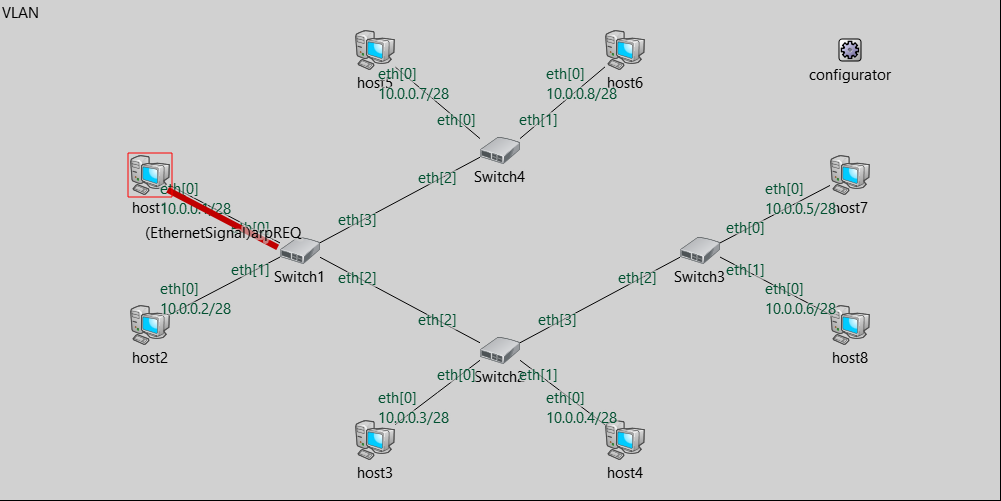
\includegraphics[width=\linewidth]{screenshot047}
		\end{minipage}\hfill
		\begin{minipage}{0.49\textwidth}
			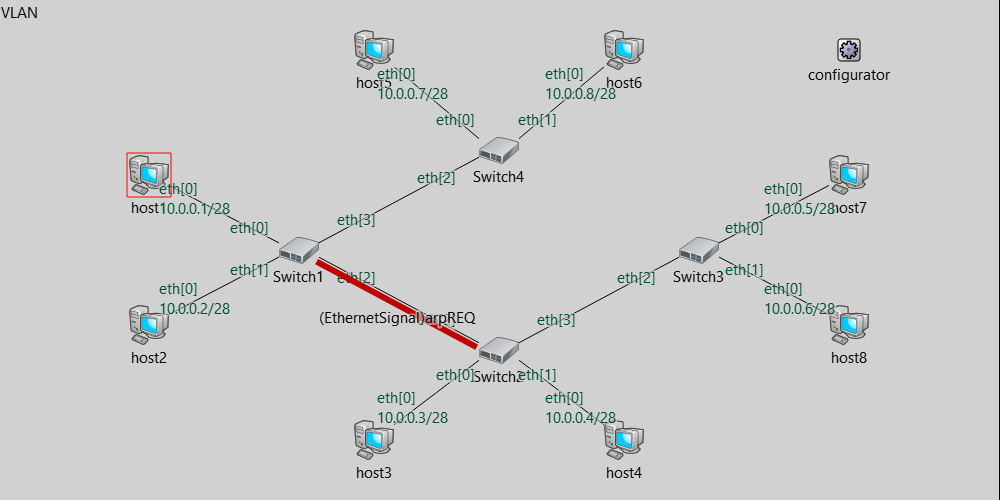
\includegraphics[width=\linewidth]{screenshot048}
		\end{minipage}\hfill
	\end{figure}
	\begin{figure}[!htb]
		\begin{minipage}{0.49\textwidth}
			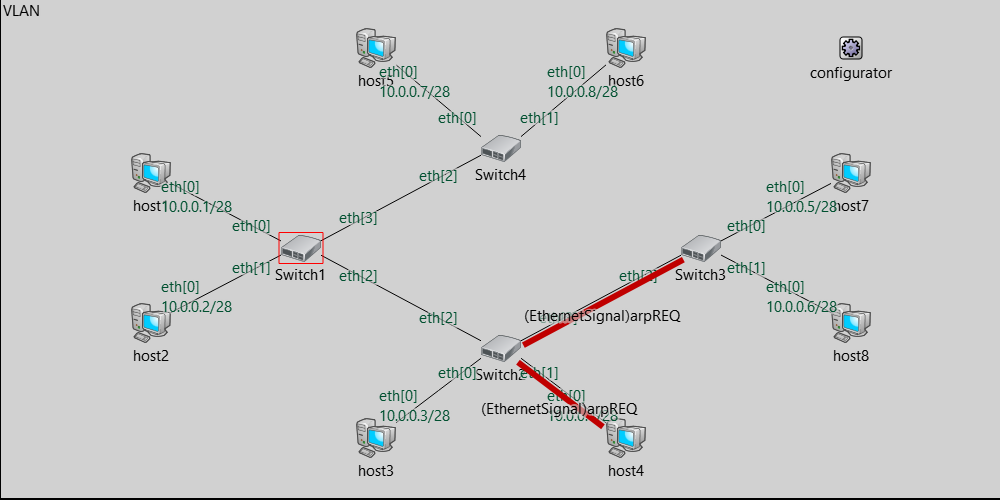
\includegraphics[width=\linewidth]{screenshot049}
		\end{minipage}\hfill
		\begin{minipage}{0.49\textwidth}
			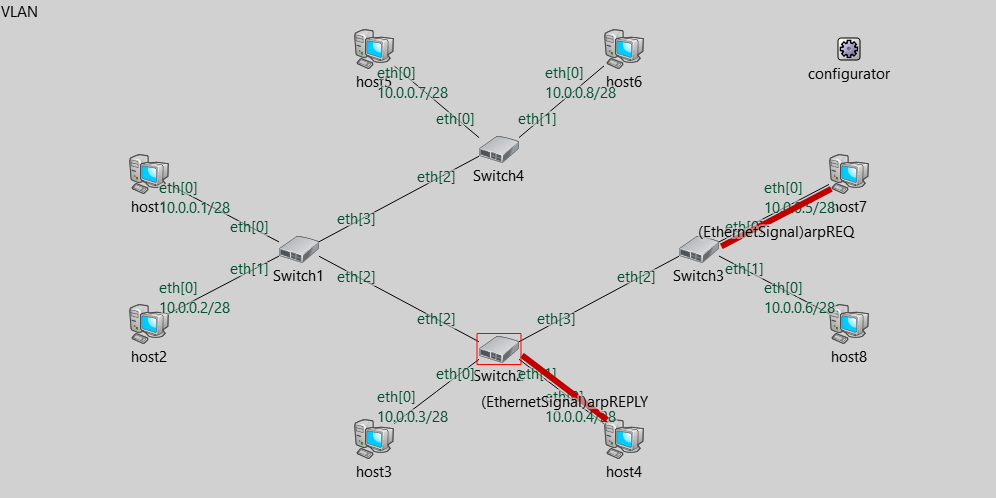
\includegraphics[width=\linewidth]{screenshot050}
		\end{minipage}\hfill
	\end{figure}
	
	\pagebreak
	
	\begin{figure}[!htb]
		\begin{minipage}{0.49\textwidth}
			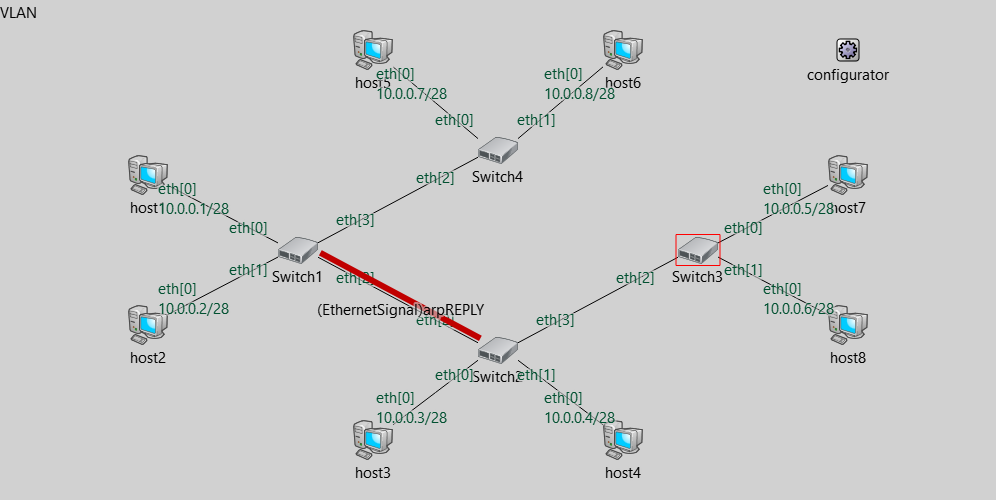
\includegraphics[width=\linewidth]{screenshot051}
		\end{minipage}\hfill
		\begin{minipage}{0.49\textwidth}
			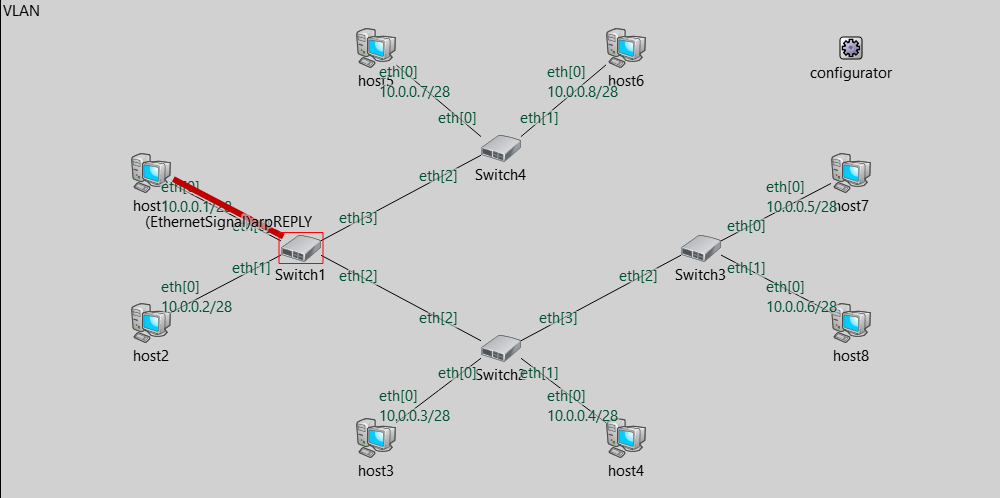
\includegraphics[width=\linewidth]{screenshot052}
		\end{minipage}\hfill
	\end{figure}
	\begin{figure}[!htb]
		\begin{minipage}{0.49\textwidth}
			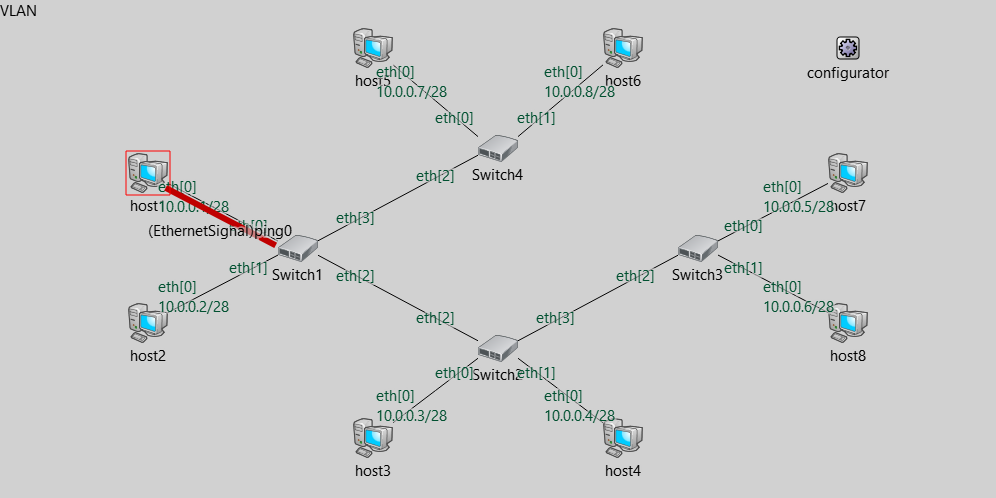
\includegraphics[width=\linewidth]{screenshot053}
		\end{minipage}\hfill
		\begin{minipage}{0.49\textwidth}
			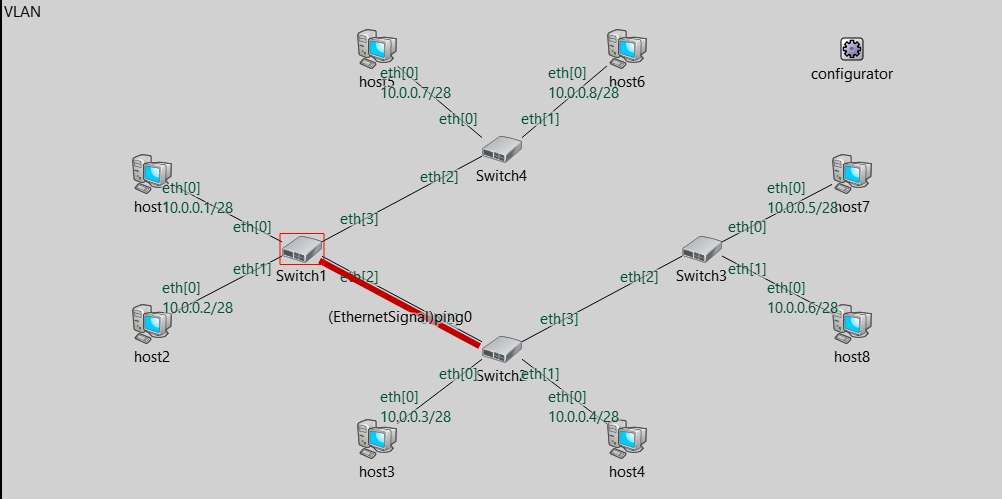
\includegraphics[width=\linewidth]{screenshot054}
		\end{minipage}\hfill
	\end{figure}
	\begin{figure}[!htb]
		\begin{minipage}{0.49\textwidth}
			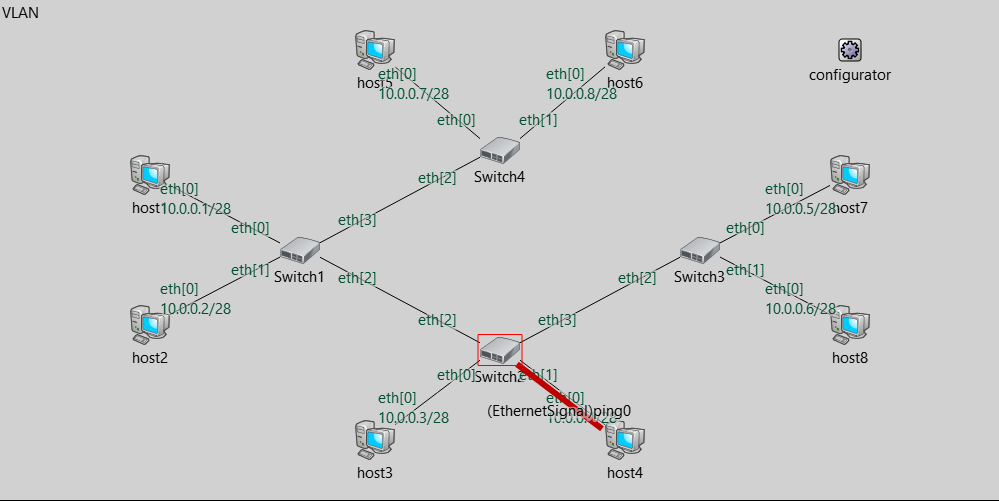
\includegraphics[width=\linewidth]{screenshot055}
		\end{minipage}\hfill
		\begin{minipage}{0.49\textwidth}
			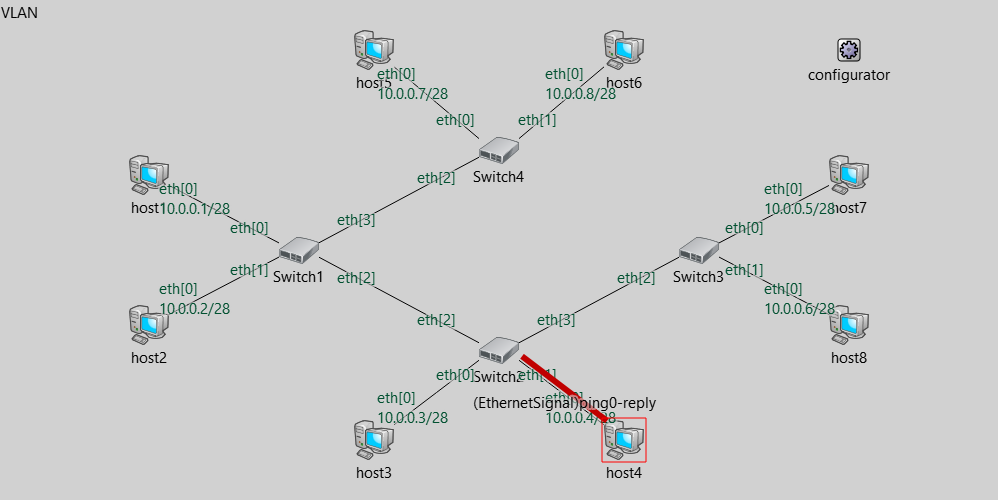
\includegraphics[width=\linewidth]{screenshot056}
		\end{minipage}\hfill
	\end{figure}
	\begin{figure}[!htb]
		\begin{minipage}{0.49\textwidth}
			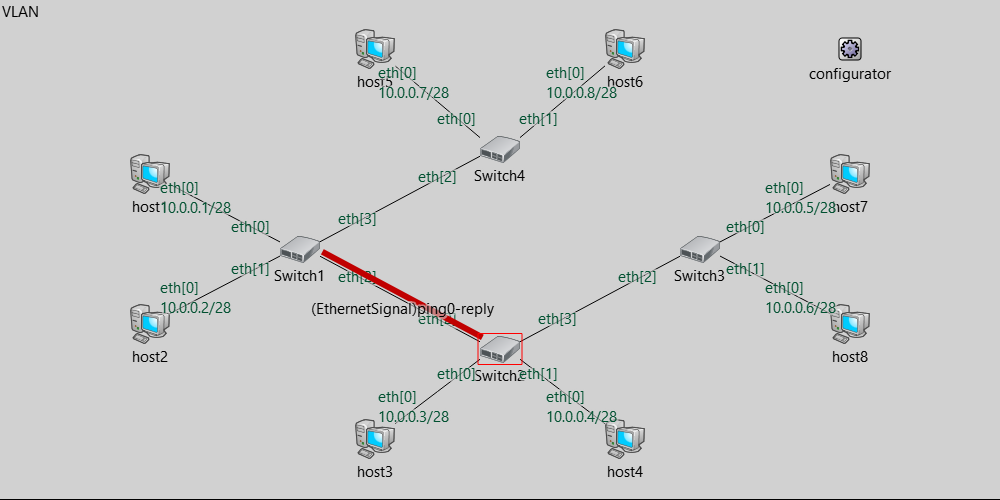
\includegraphics[width=\linewidth]{screenshot057}
		\end{minipage}\hfill
		\begin{minipage}{0.49\textwidth}
			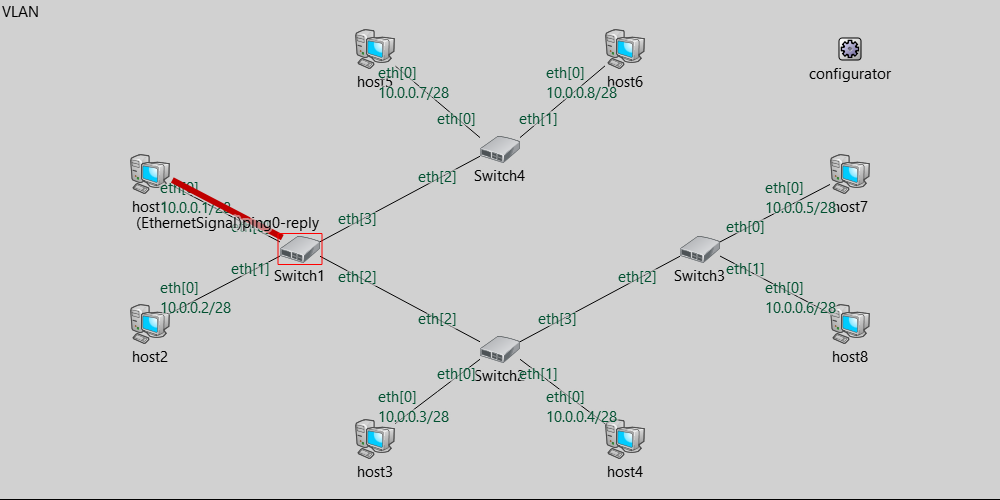
\includegraphics[width=\linewidth]{screenshot058}
		\end{minipage}\hfill
	\end{figure}
	
	\pagebreak
	
	\begin{center}
		packet flow for \textit{host8} $\rightarrow$ \textit{host6} communication
	\end{center}
	
	\begin{figure}[!htb]
		\begin{minipage}{0.49\textwidth}
			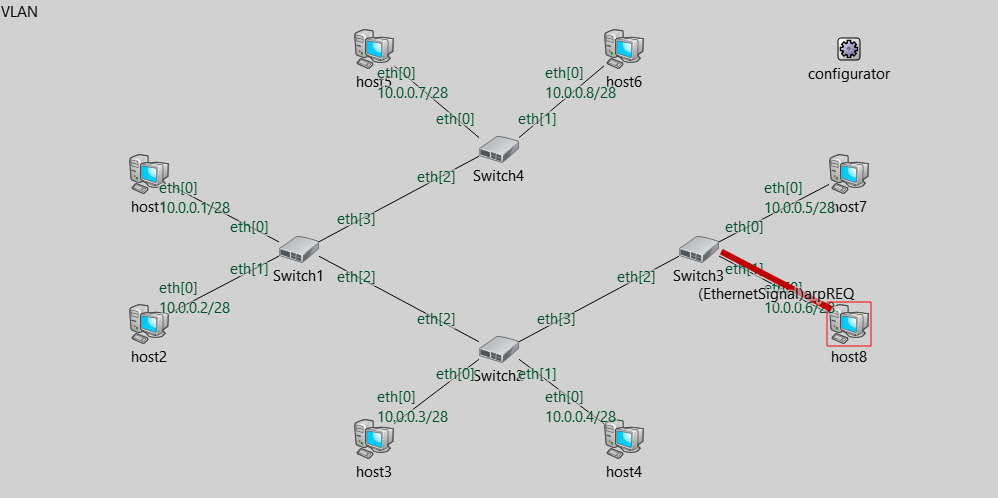
\includegraphics[width=\linewidth]{screenshot059}
		\end{minipage}\hfill
		\begin{minipage}{0.49\textwidth}
			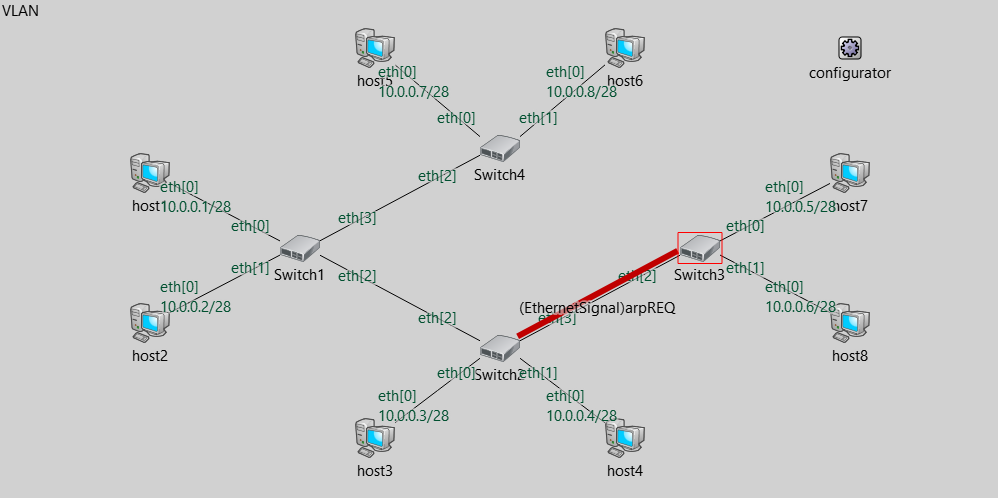
\includegraphics[width=\linewidth]{screenshot060}
		\end{minipage}\hfill
	\end{figure}
	\begin{figure}[!htb]
		\begin{minipage}{0.49\textwidth}
			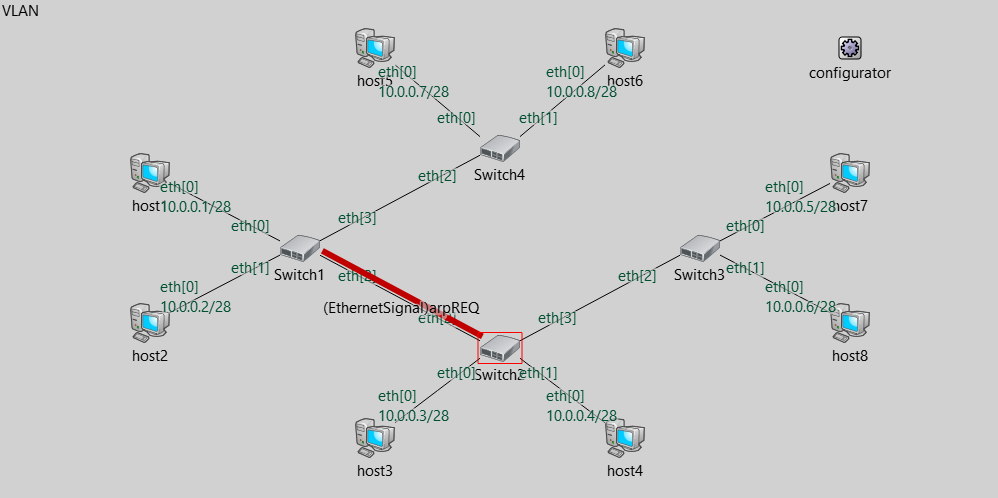
\includegraphics[width=\linewidth]{screenshot061}
		\end{minipage}\hfill
		\begin{minipage}{0.49\textwidth}
			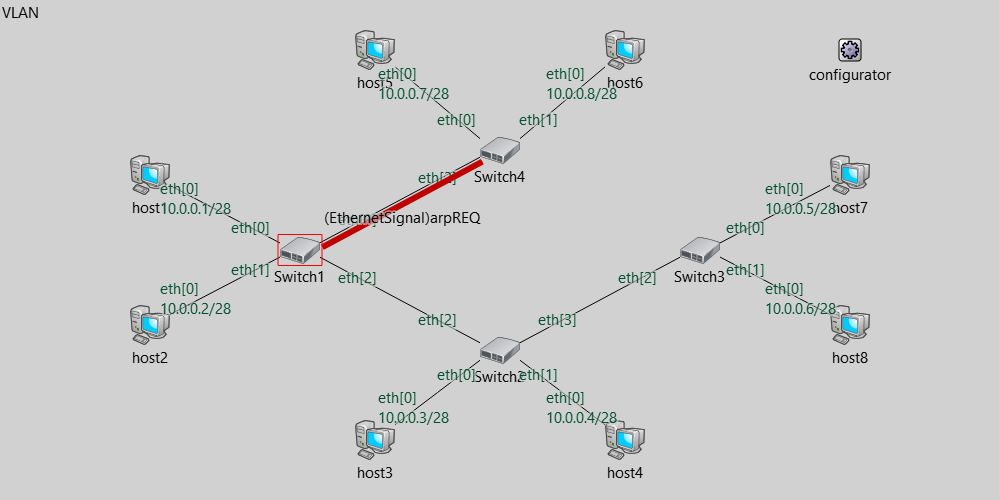
\includegraphics[width=\linewidth]{screenshot062}
		\end{minipage}\hfill
	\end{figure}
	\begin{figure}[!htb]
		\begin{minipage}{0.49\textwidth}
			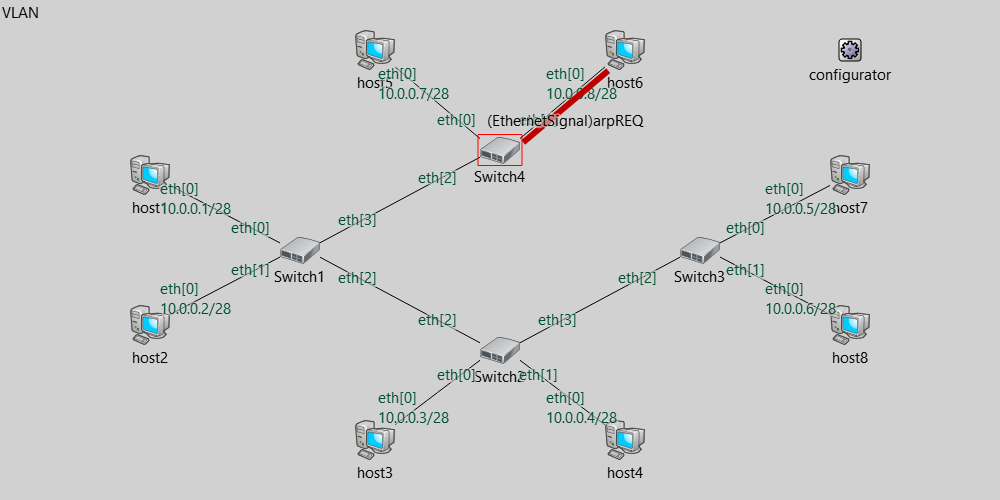
\includegraphics[width=\linewidth]{screenshot063}
		\end{minipage}\hfill
		\begin{minipage}{0.49\textwidth}
			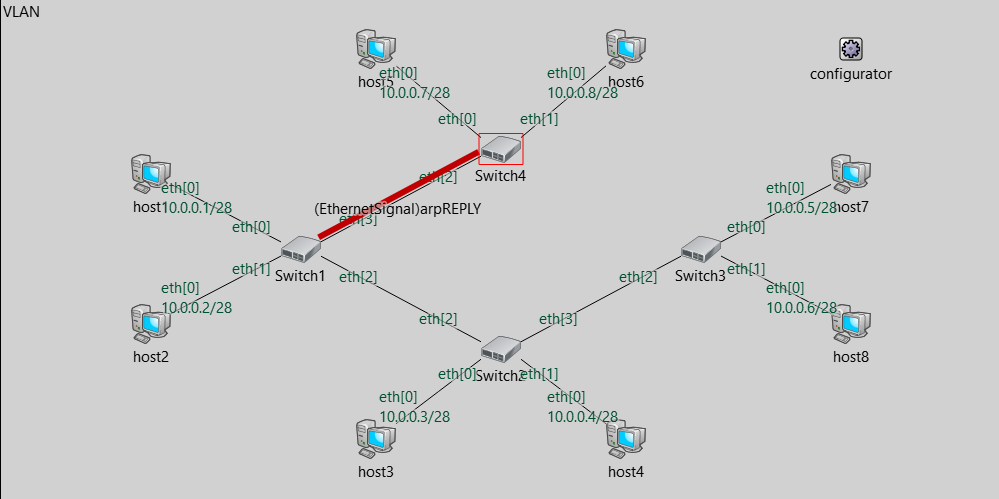
\includegraphics[width=\linewidth]{screenshot064}
		\end{minipage}\hfill
	\end{figure}
	\begin{figure}[!htb]
		\begin{minipage}{0.49\textwidth}
			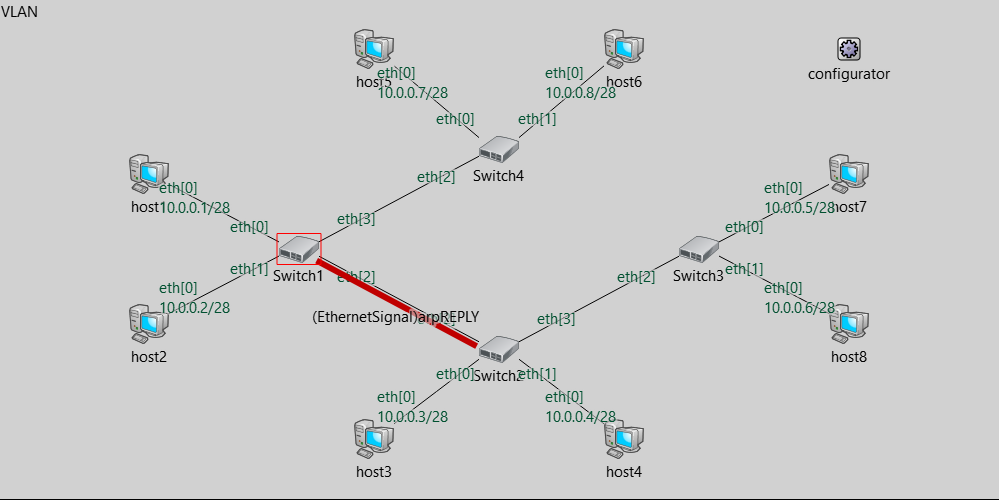
\includegraphics[width=\linewidth]{screenshot065}
		\end{minipage}\hfill
		\begin{minipage}{0.49\textwidth}
			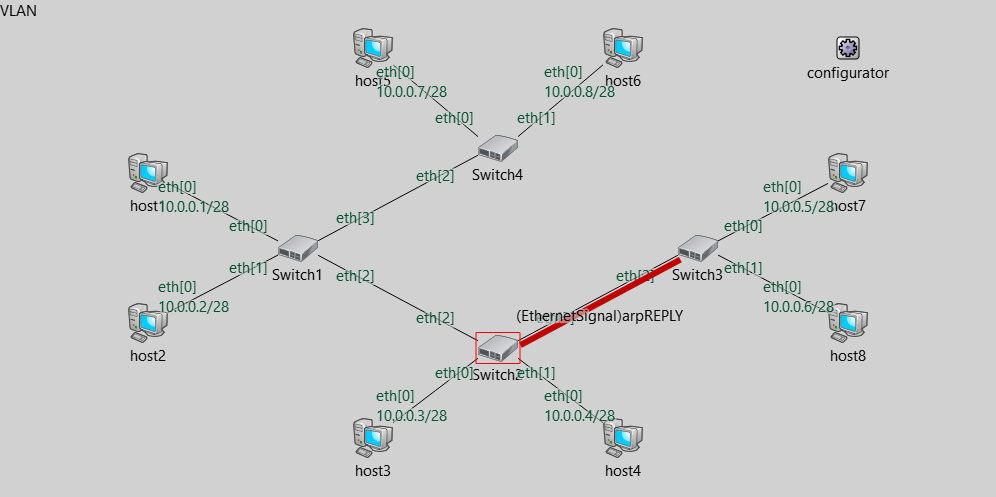
\includegraphics[width=\linewidth]{screenshot066}
		\end{minipage}\hfill
	\end{figure}
	\begin{figure}[!htb]
		\begin{minipage}{0.49\textwidth}
			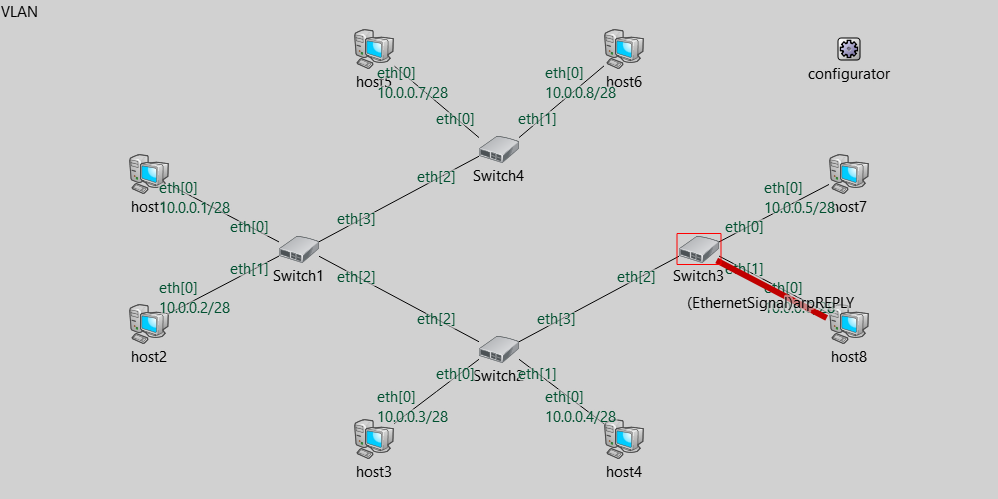
\includegraphics[width=\linewidth]{screenshot067}
		\end{minipage}\hfill
		\begin{minipage}{0.49\textwidth}
			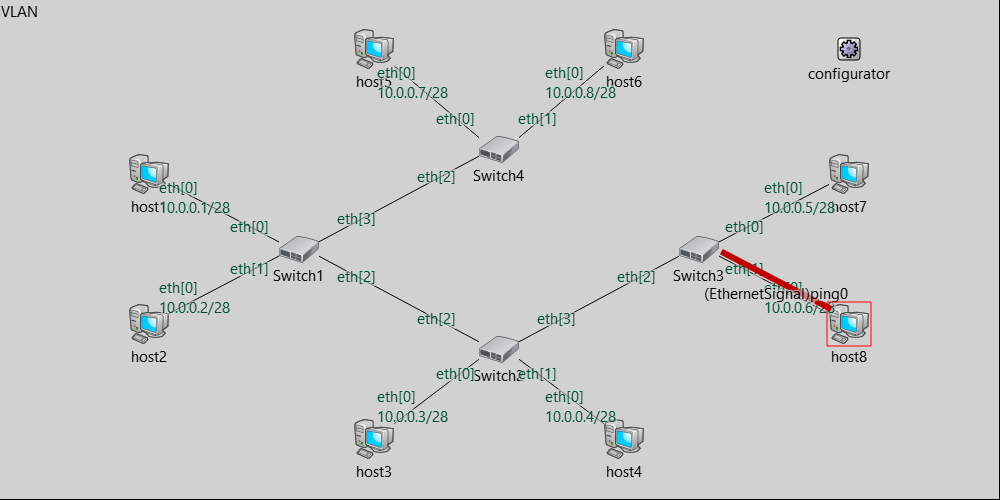
\includegraphics[width=\linewidth]{screenshot068}
		\end{minipage}\hfill
	\end{figure}
	
	\pagebreak
	
	\begin{figure}[!htb]
		\begin{minipage}{0.49\textwidth}
			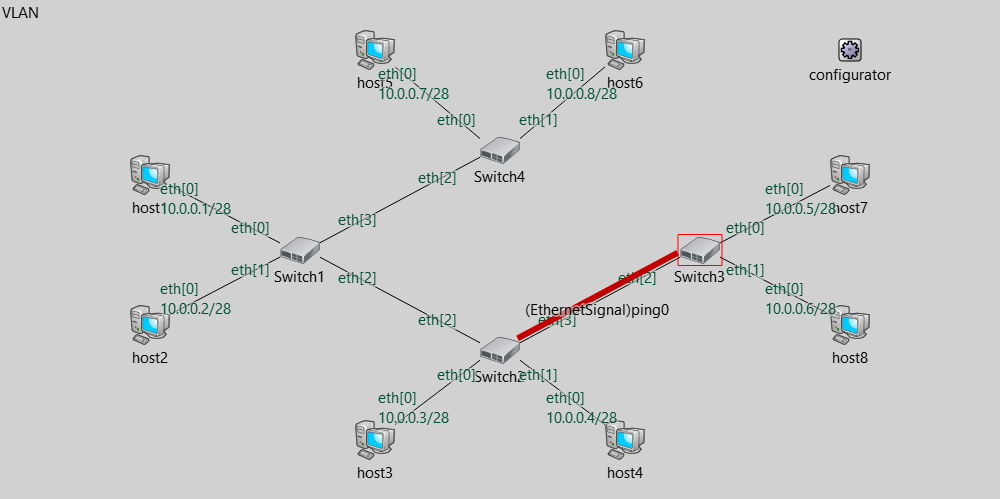
\includegraphics[width=\linewidth]{screenshot069}
		\end{minipage}\hfill
		\begin{minipage}{0.49\textwidth}
			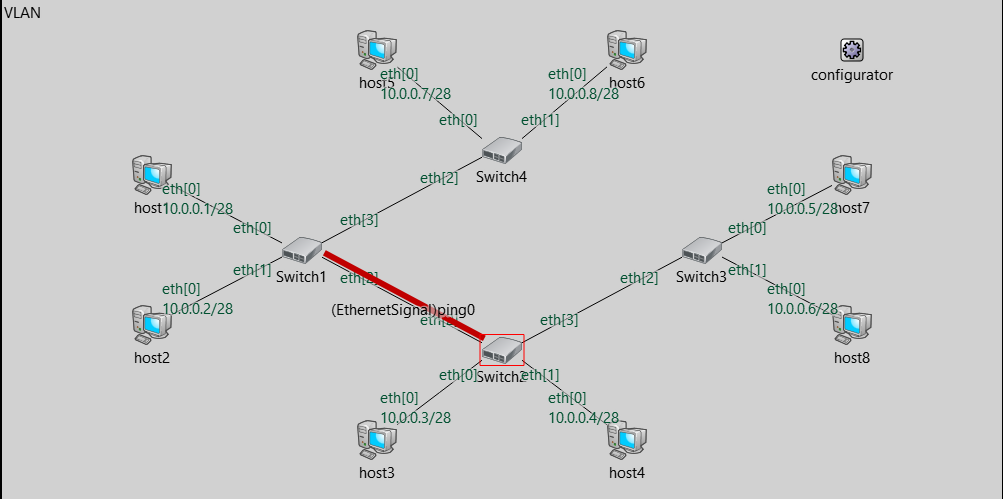
\includegraphics[width=\linewidth]{screenshot070}
		\end{minipage}\hfill
	\end{figure}
	\begin{figure}[!htb]
		\begin{minipage}{0.49\textwidth}
			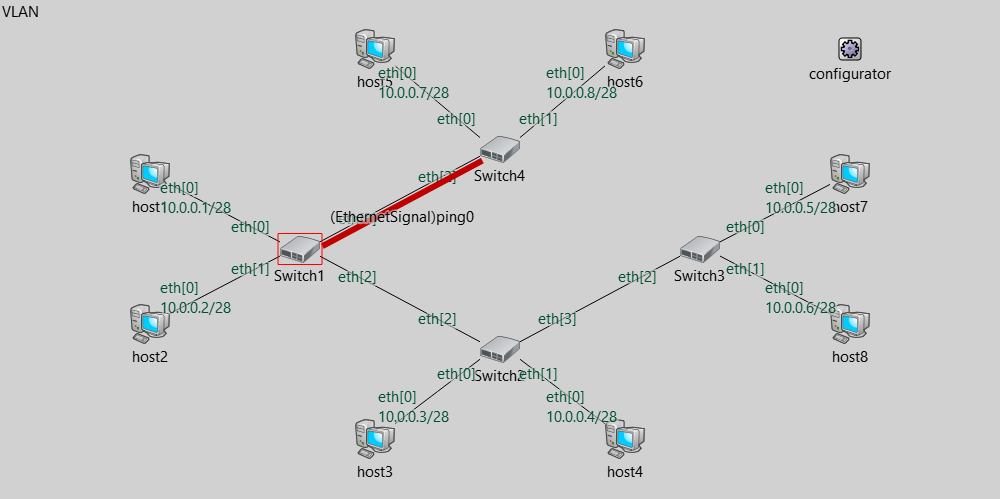
\includegraphics[width=\linewidth]{screenshot071}
		\end{minipage}\hfill
		\begin{minipage}{0.49\textwidth}
			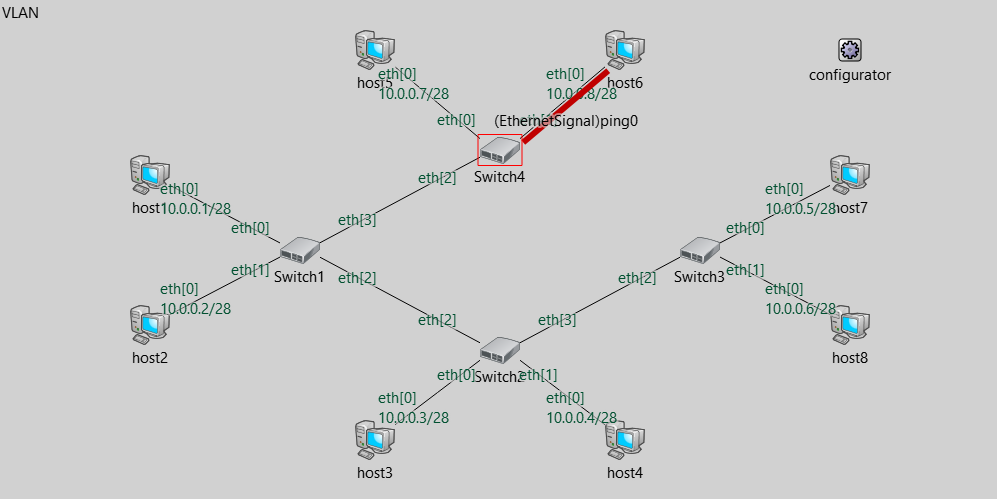
\includegraphics[width=\linewidth]{screenshot072}
		\end{minipage}\hfill
	\end{figure}
	\begin{figure}[!htb]
		\begin{minipage}{0.49\textwidth}
			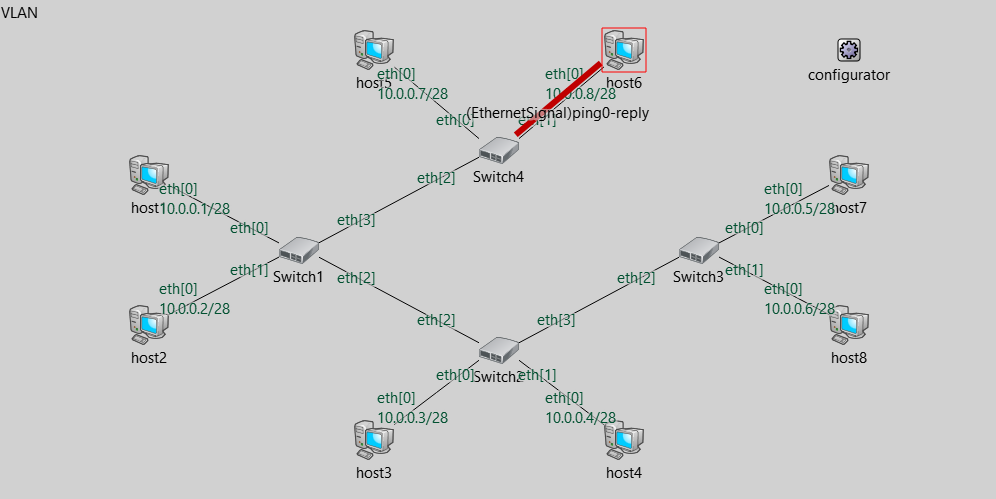
\includegraphics[width=\linewidth]{screenshot073}
		\end{minipage}\hfill
		\begin{minipage}{0.49\textwidth}
			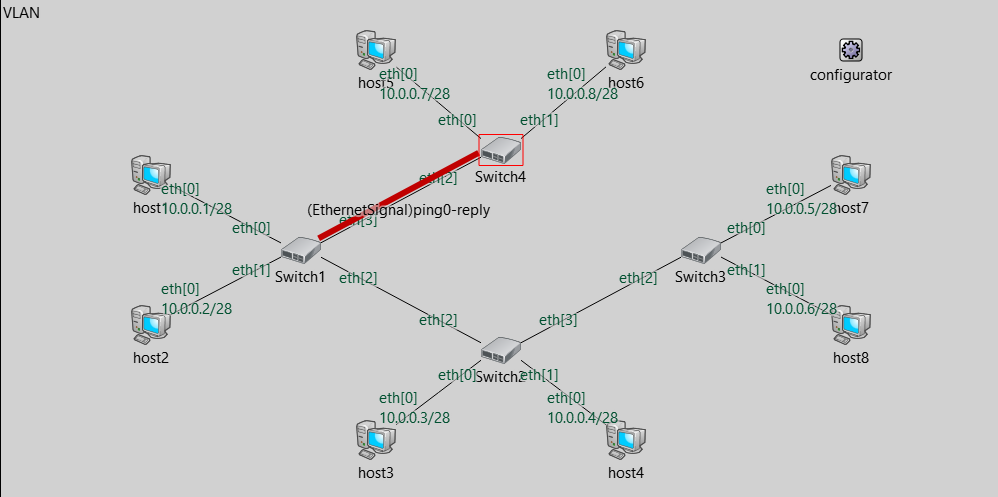
\includegraphics[width=\linewidth]{screenshot074}
		\end{minipage}\hfill
	\end{figure}
	\begin{figure}[!htb]
		\begin{minipage}{0.49\textwidth}
			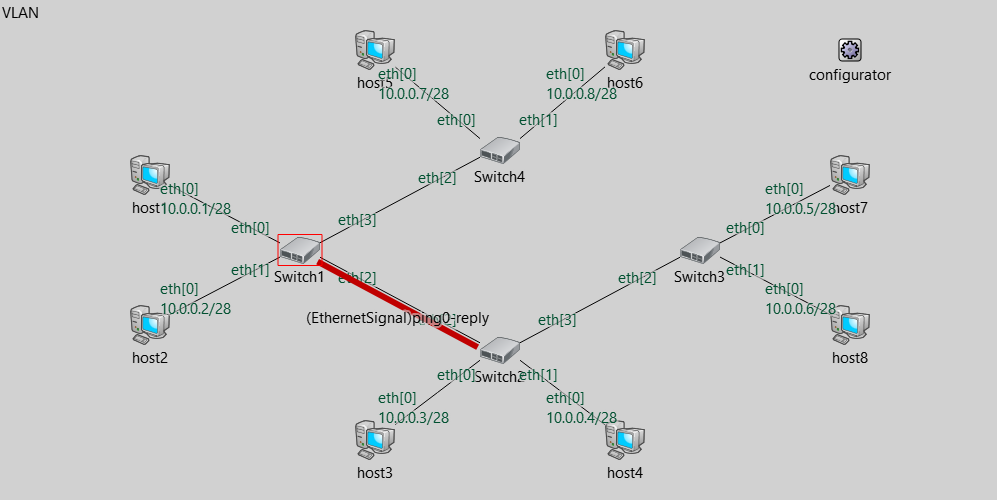
\includegraphics[width=\linewidth]{screenshot075}
		\end{minipage}\hfill
		\begin{minipage}{0.49\textwidth}
			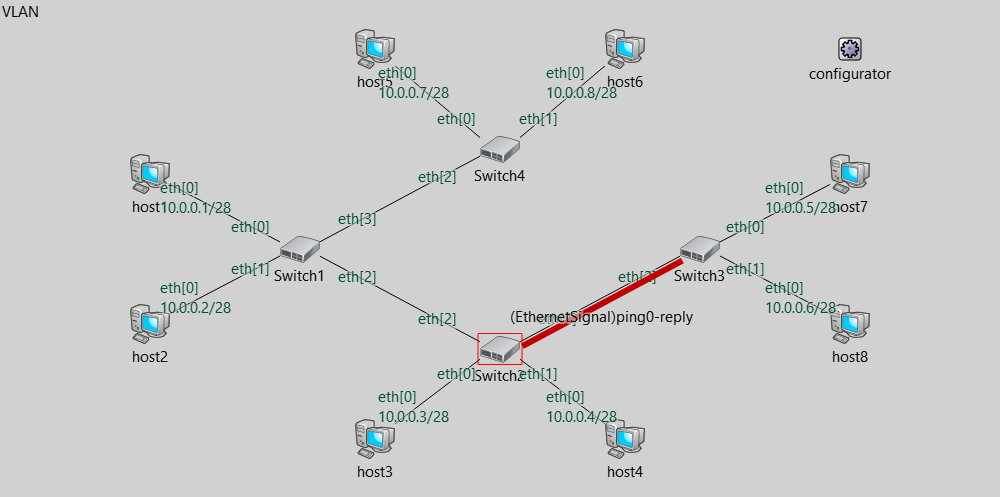
\includegraphics[width=\linewidth]{screenshot076}
		\end{minipage}\hfill
	\end{figure}
	
	As you can see from the results, the source hosts first send a packet named \textit{arpREQ} to the destination hosts to find the MAC address of the destination host in order to transmit the data.
	
	After the reply from the destination came back to the source host, it starts to send \textit{ping} packets to the known destination.
	
	We note that the \textit{arpREQ} packets are sent from every port of each switch than allows transmission of a vlanID similar to the one used in the source host. For example the \textit{arpREQ} packet from \textit{host1} to \textit{host4} is sent from \textit{Switch1} only to \textit{Switch2} because \textit{Switch4} only allows VLANs 20 and 30.
	
	The other thing worth of noting is that after learning the MAC address of the destination and source hosts, the switches only send packets in the correct paths to source and destination and do not send the packets to all nodes accepting packets having valid vlanIDs.
	
	\pagebreak
	
	\Large
	e)
	\large
	
	In the following figures I have captured the flow of the traffic moved between \textit{host1} and \textit{host7}. 
	
	\begin{center}
		\textit{arpREQ} packet transmission
	\end{center}
	
	\begin{figure}[!htb]
		\begin{minipage}{0.49\textwidth}
			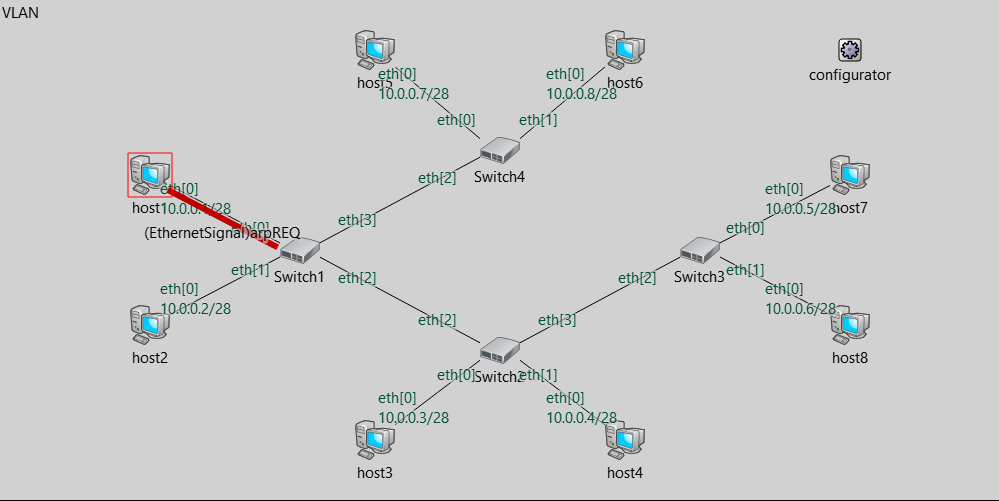
\includegraphics[width=\linewidth]{screenshot078}
		\end{minipage}\hfill
		\begin{minipage}{0.49\textwidth}
			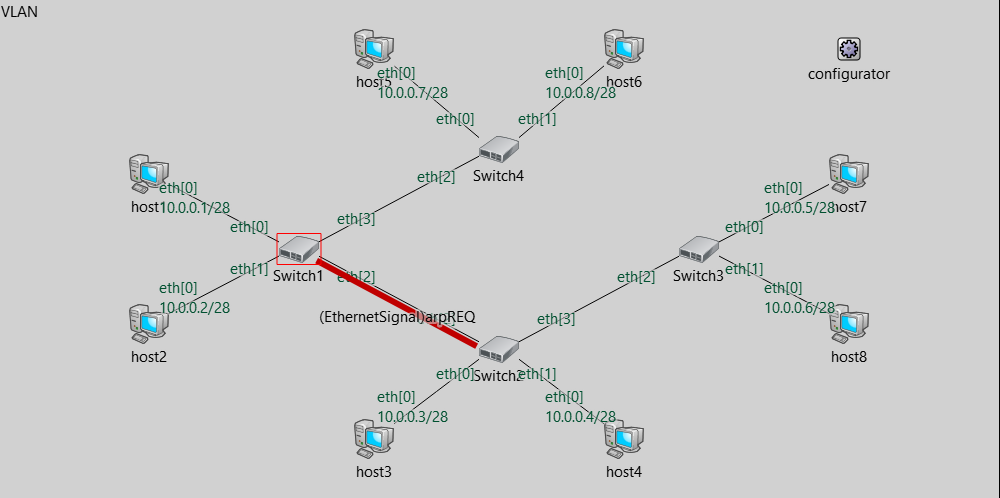
\includegraphics[width=\linewidth]{screenshot079}
		\end{minipage}\hfill
	\end{figure}
	\begin{figure}[!htb]
		\begin{minipage}{0.49\textwidth}
			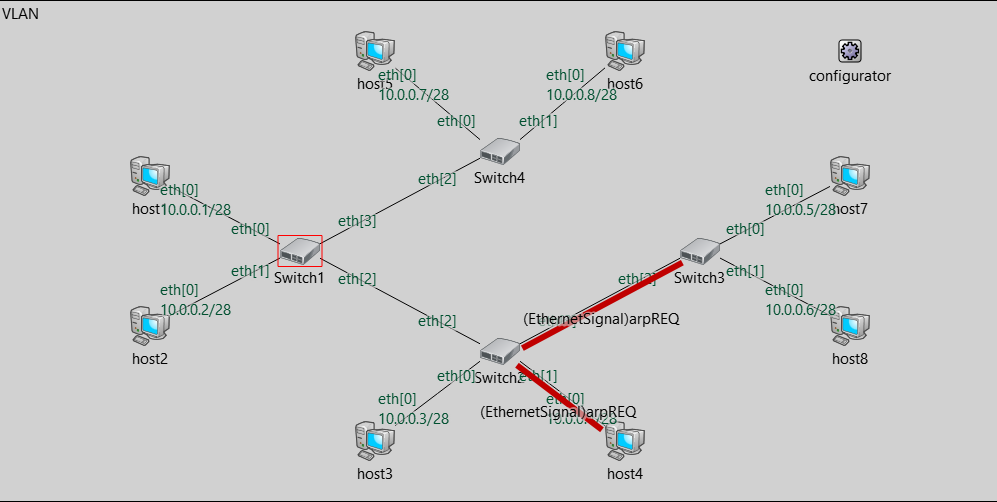
\includegraphics[width=\linewidth]{screenshot080}
		\end{minipage}\hfill
		\begin{minipage}{0.49\textwidth}
			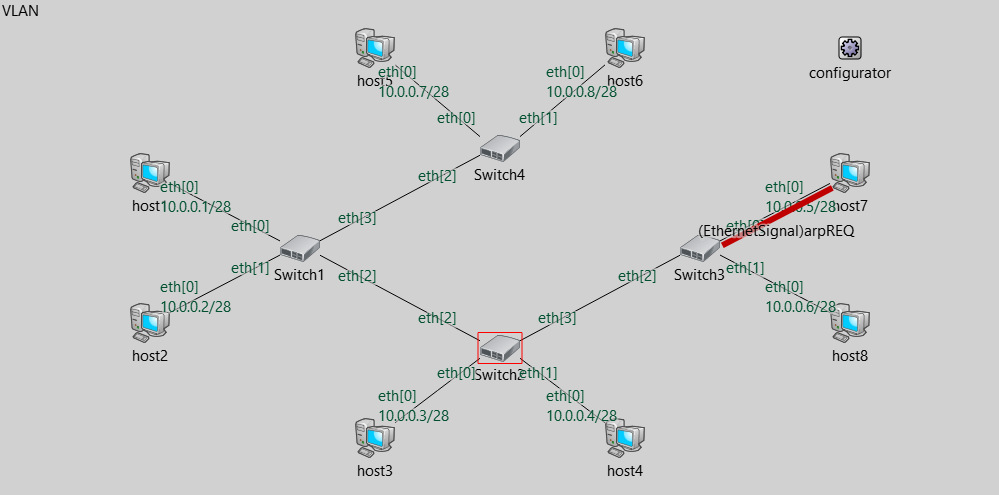
\includegraphics[width=\linewidth]{screenshot081}
		\end{minipage}\hfill
	\end{figure}
	\begin{figure}[!htb]
		\begin{minipage}{0.49\textwidth}
			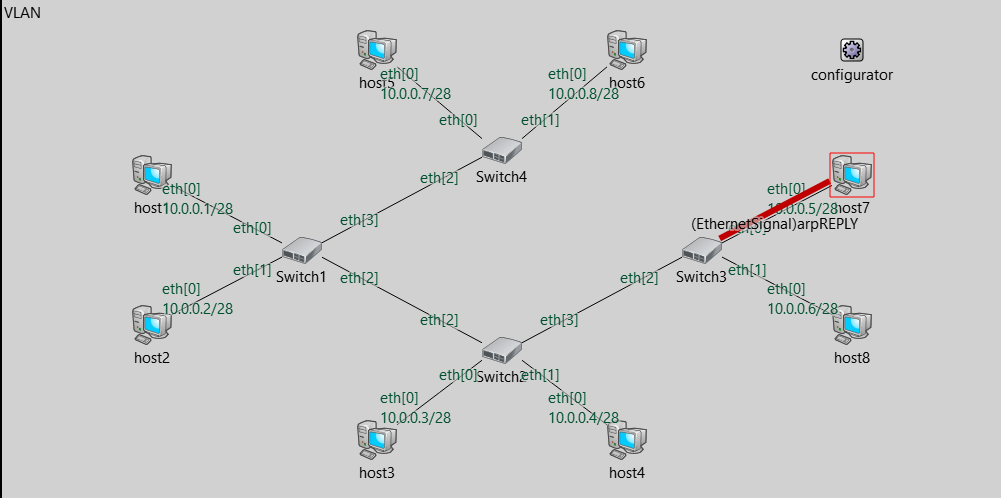
\includegraphics[width=\linewidth]{screenshot082}
		\end{minipage}\hfill
		\begin{minipage}{0.49\textwidth}
			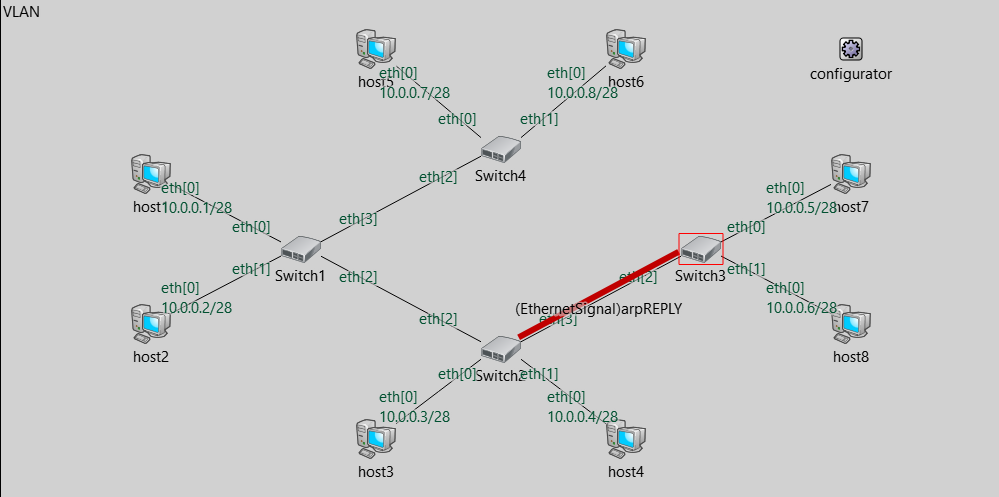
\includegraphics[width=\linewidth]{screenshot083}
		\end{minipage}\hfill
	\end{figure}
	\begin{figure}[!htb]
		\begin{minipage}{0.49\textwidth}
			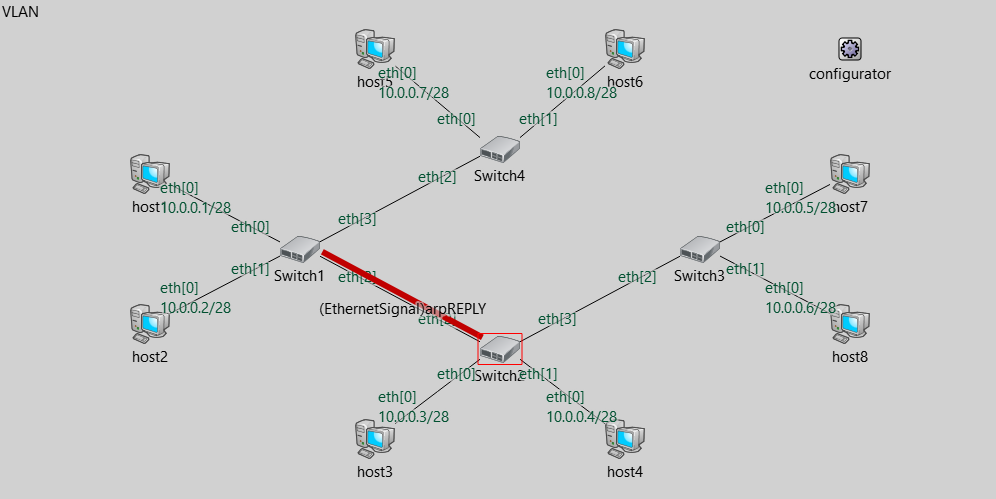
\includegraphics[width=\linewidth]{screenshot084}
		\end{minipage}\hfill
		\begin{minipage}{0.49\textwidth}
			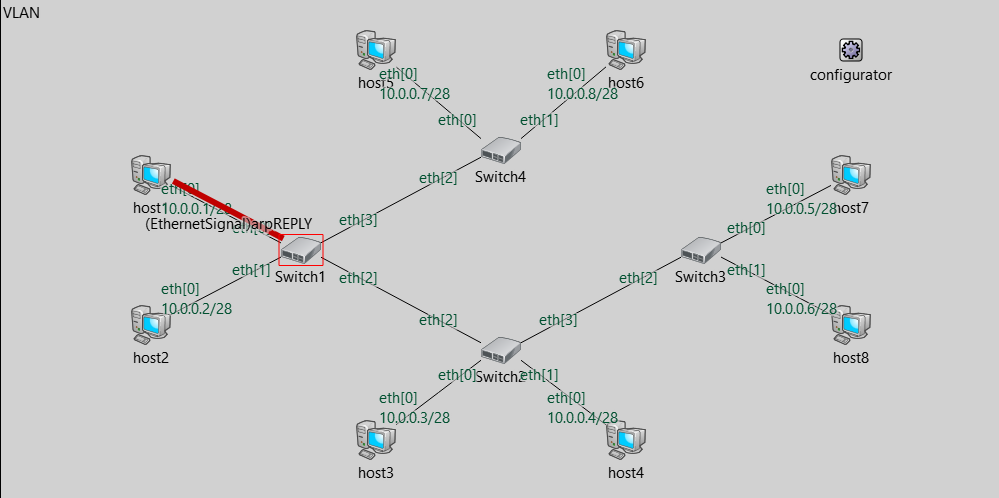
\includegraphics[width=\linewidth]{screenshot085}
		\end{minipage}\hfill
	\end{figure}
	
	nodes and switches receiving \textit{arpREQ} and \textit{arpREPLY} packets:
	\begin{center}
		\textit{host1} \quad,\quad \textit{Switch1} \quad,\quad \textit{Switch2} \quad,\quad \textit{host4} \quad,\quad \textit{Switch3} \quad,\quad \textit{host7}
	\end{center}
	note that \textit{host1} and \textit{host4} receive only \textit{arpREPLY} and \textit{arpREQ} respectively.
	
	\pagebreak
	
	\begin{center}
		\textit{ping} packet transmission
	\end{center}
	
	\begin{figure}[!htb]
		\begin{minipage}{0.49\textwidth}
			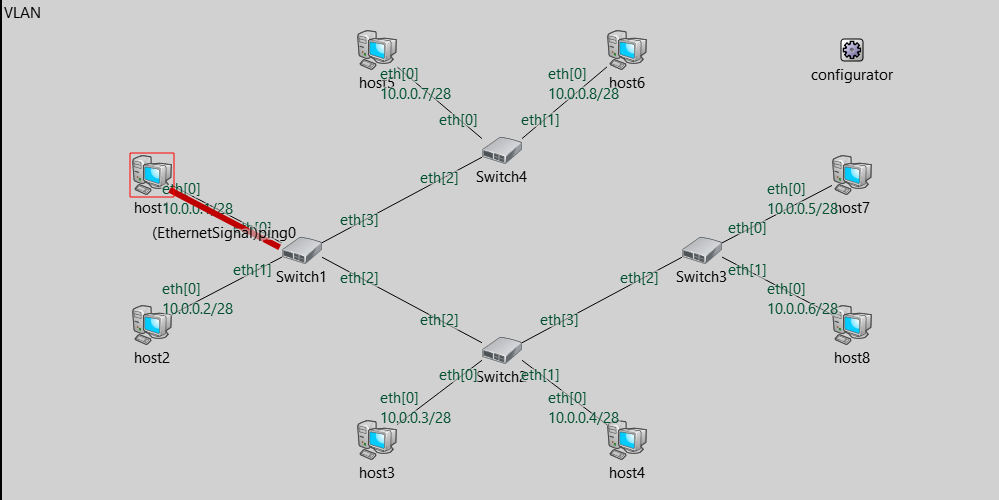
\includegraphics[width=\linewidth]{screenshot086}
		\end{minipage}\hfill
		\begin{minipage}{0.49\textwidth}
			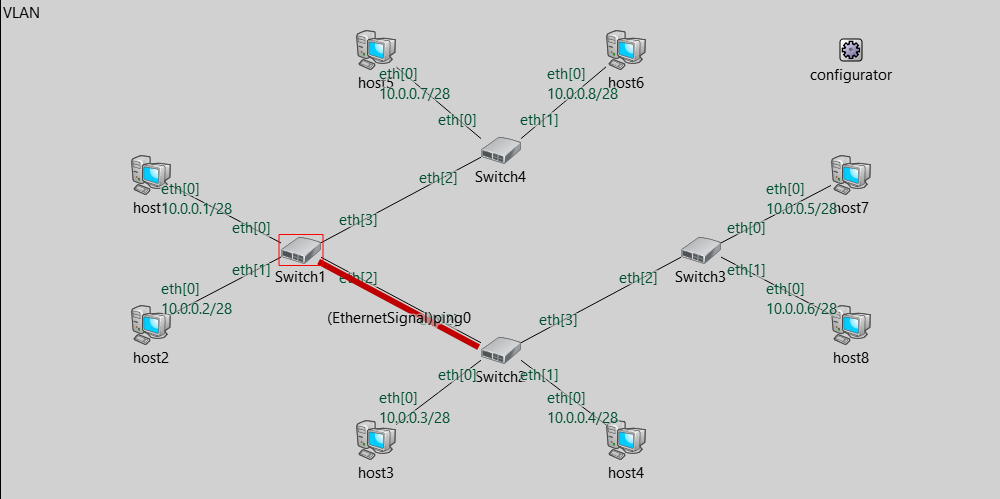
\includegraphics[width=\linewidth]{screenshot087}
		\end{minipage}\hfill
	\end{figure}
	\begin{figure}[!htb]
		\begin{minipage}{0.49\textwidth}
			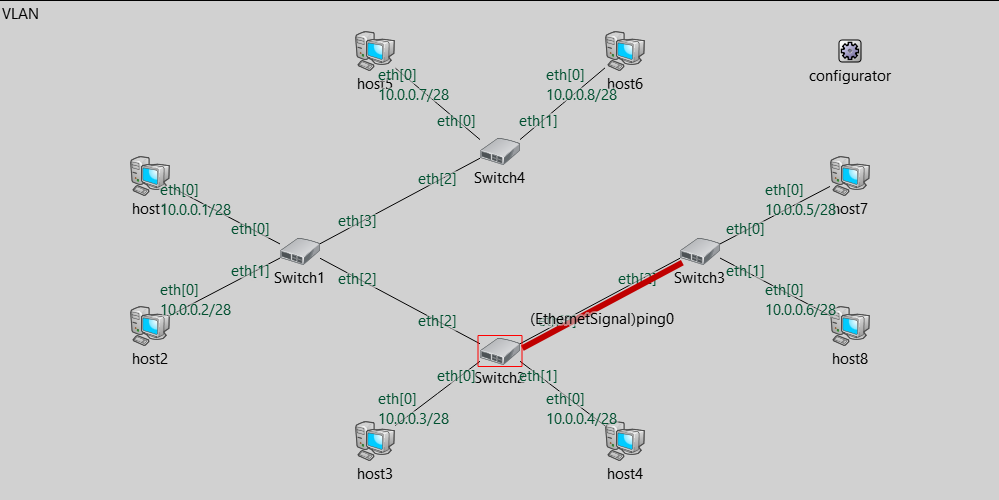
\includegraphics[width=\linewidth]{screenshot088}
		\end{minipage}\hfill
		\begin{minipage}{0.49\textwidth}
			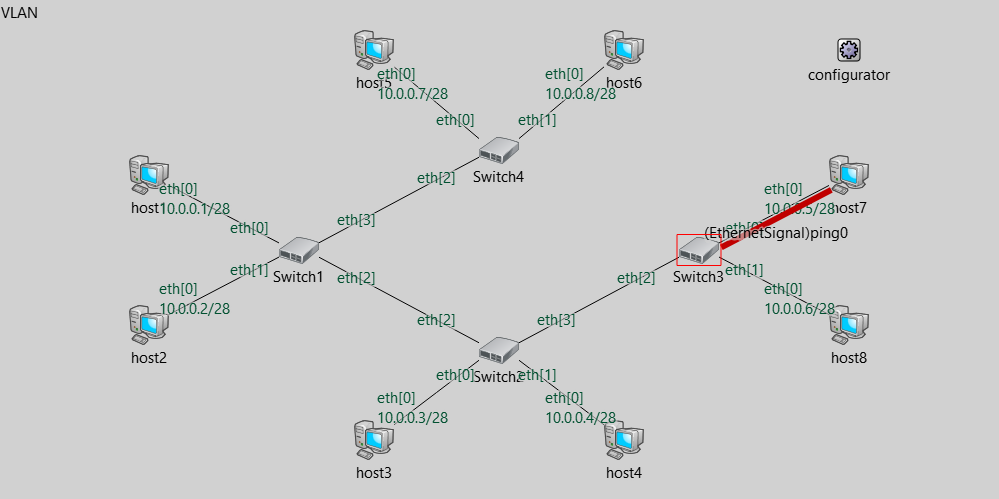
\includegraphics[width=\linewidth]{screenshot089}
		\end{minipage}\hfill
	\end{figure}
	\begin{figure}[!htb]
		\begin{minipage}{0.49\textwidth}
			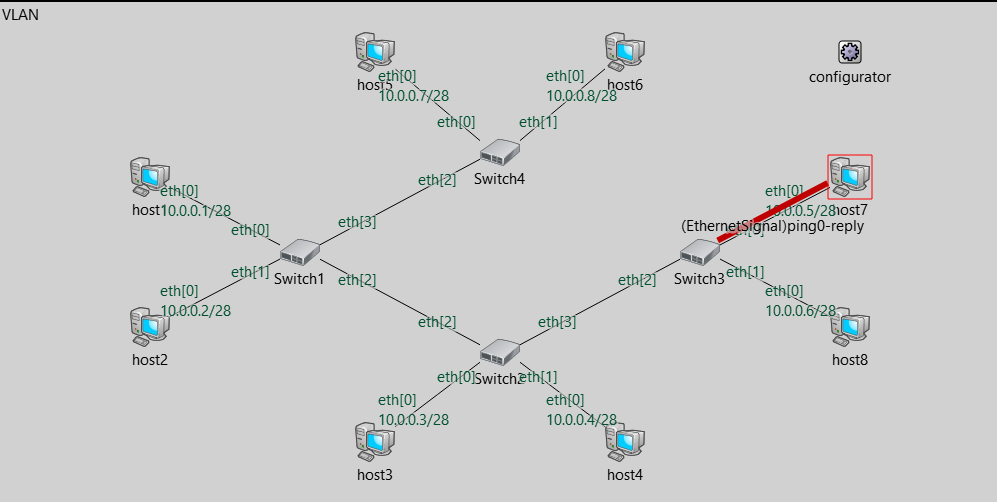
\includegraphics[width=\linewidth]{screenshot090}
		\end{minipage}\hfill
		\begin{minipage}{0.49\textwidth}
			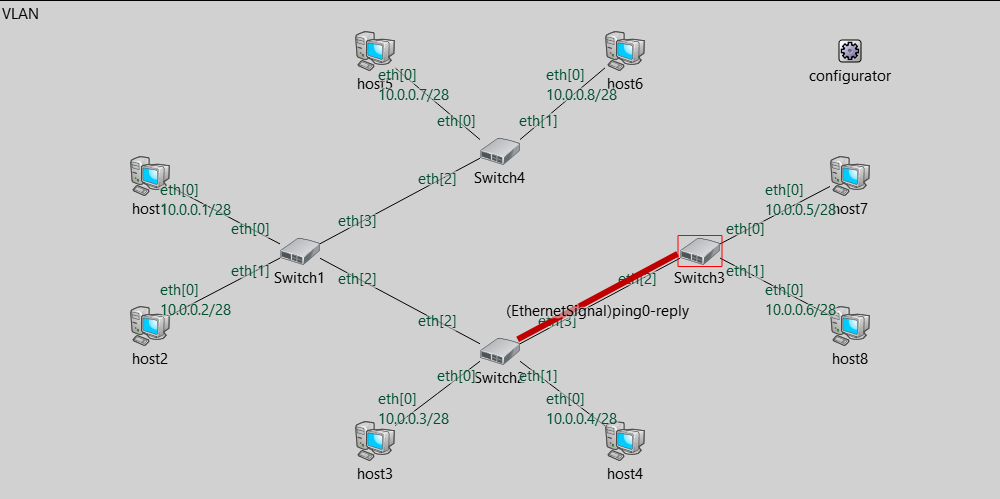
\includegraphics[width=\linewidth]{screenshot091}
		\end{minipage}\hfill
	\end{figure}
	\begin{figure}[!htb]
		\begin{minipage}{0.49\textwidth}
			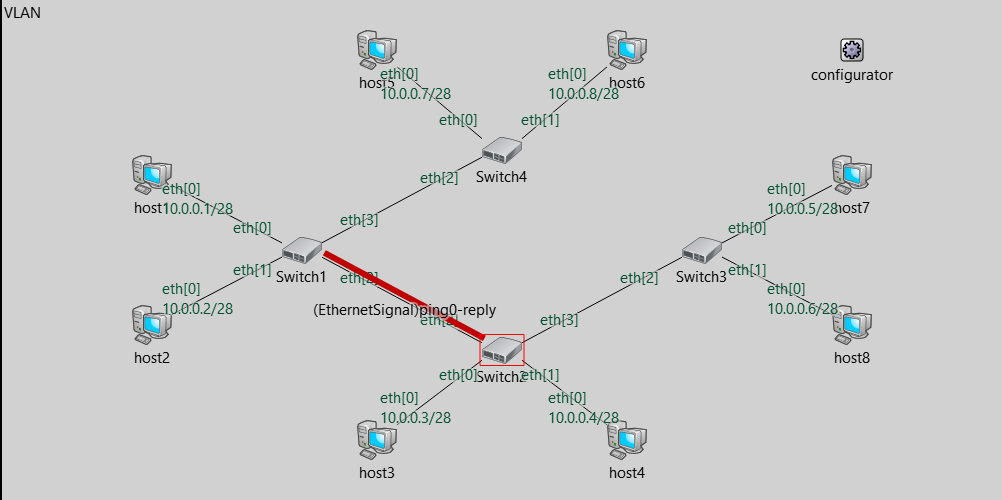
\includegraphics[width=\linewidth]{screenshot092}
		\end{minipage}\hfill
		\begin{minipage}{0.49\textwidth}
			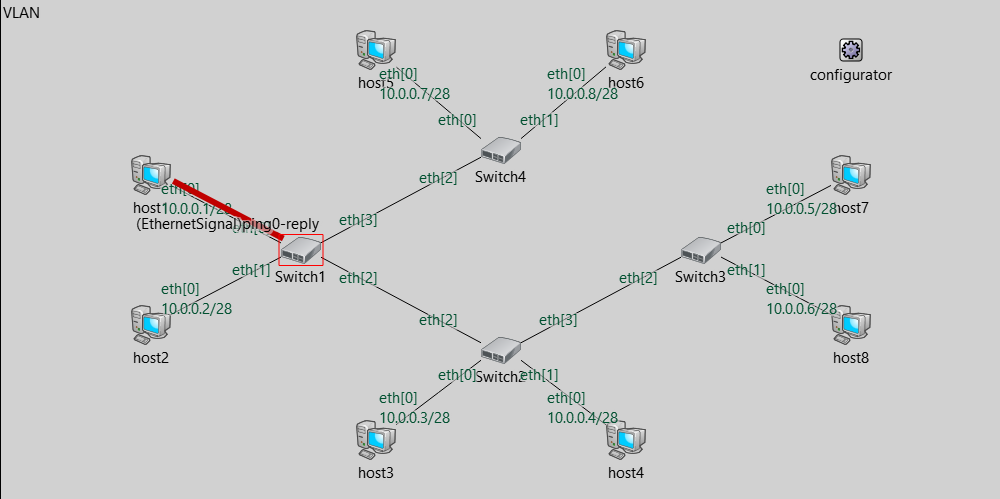
\includegraphics[width=\linewidth]{screenshot093}
		\end{minipage}\hfill
	\end{figure}
	
	nodes and switches receiving \textit{ping} packets:
	\begin{center}
		\textit{Switch1} \qquad,\qquad \textit{Switch2} \qquad,\qquad \textit{Switch3} \qquad,\qquad \textit{host7}
	\end{center}
	
	\pagebreak
	
	ARP (Address Resolution Protocol) is used to map an IP address to a MAC address in a local network. When a host wants to send data to another host on the same local network, it needs to know the MAC address of the destination host. While the IP address uniquely identifies a host on the network, only the MAC address can be used for actual data transfer on the local link.
	
	When a host wants to communicate with another host on the same network, it checks its ARP cache (a table where the device keeps a record of known IP-to-MAC address mappings).
	
	If the IP address of the destination host is not found in the ARP cache, an \textit{arpREQ} is sent out.
	
	This request is a broadcast message sent to all host on the local network (since the sender doesn't know the destination device's MAC address).
	
	The \textit{arpREQ} contains the sender’s IP and MAC address and asks:
	\begin{center}
		"Who has this IP address? Please reply with your MAC address."
	\end{center}
	The device that owns the IP address in the \textit{arpREQ} responds with an \textit{arpREPLY} which includes its MAC address.
	
	The sender then stores this mapping (IP-to-MAC address) in its ARP cache so future communications to this IP can be sent directly to the MAC address without needing another \textit{arpREQ}.
	
	Therefore the \textit{arpREQ} packets precede \textit{ping} packets because the source needs to find out what the MAC address of the destination host is in order to sent data and communicate.
	
\end{document}